\section{Projeto da Biblioteca} \label{sec:projeto}

\subsection{Levantamento de requisitos}
Realizando reuniões semanais com professores envolvidos no projeto, além de apresentar à outros professores que possivelmente estariam interessados no projeto, foi utilizado a técnica de \emph{brainstorm} para o levantamento de requisitos da biblioteca.

A princípio, ela deveria ser aplicada em cada tópico abordado em \acrshort{APC}, sendo utilizada de forma lúdica e didática do início ao final do semestre. A biblioteca deve ser capaz de acompanhar a evolução gradativa de complexidade dos programas desenvolvidos pelos alunos.

Foram reunidos cinco grandes funcionalidades que a biblioteca deveria ter inicialmente, sendo elas: 
 \begin{itemize}
 \item Renderização de formas geométricas;
 \item Animação;
 \item Renderização de imagens;
 \item Entrada de mouse e teclado e;
 \item Outras, no intuito de auxiliar o aluno a manipular as demais funções da biblioteca;
 \end{itemize}

Sendo todas as funcionalidades capazes de serem utilizadas em qualquer período ao longo do semestre.

Com o avanço das reuniões, viu-se necessário pesquisar quais os tópicos da primeira matéria da computação em outras universidades eram abordados para a elaboração de uma apostila de exercícios (Apêndice \ref{appendix:apostila}) genérica, não apenas focada em \acrshort{APC} da \acrshort{UnB}. A Figura \ref{fig:conteudos} ilustra uma pesquisa realizada com 25 universidades, das quais foram analisados as ementas e planos de aulas (Anexo \ref{attachment:ementas}), fazendo uma relação entre os conteúdos abordados com a quantidade de universidades que os abordam. A Tabela \ref{tab:universidades} indica as universidades que foram pesquisadas.

\begin{sidewaysfigure}
  \begin{center}
    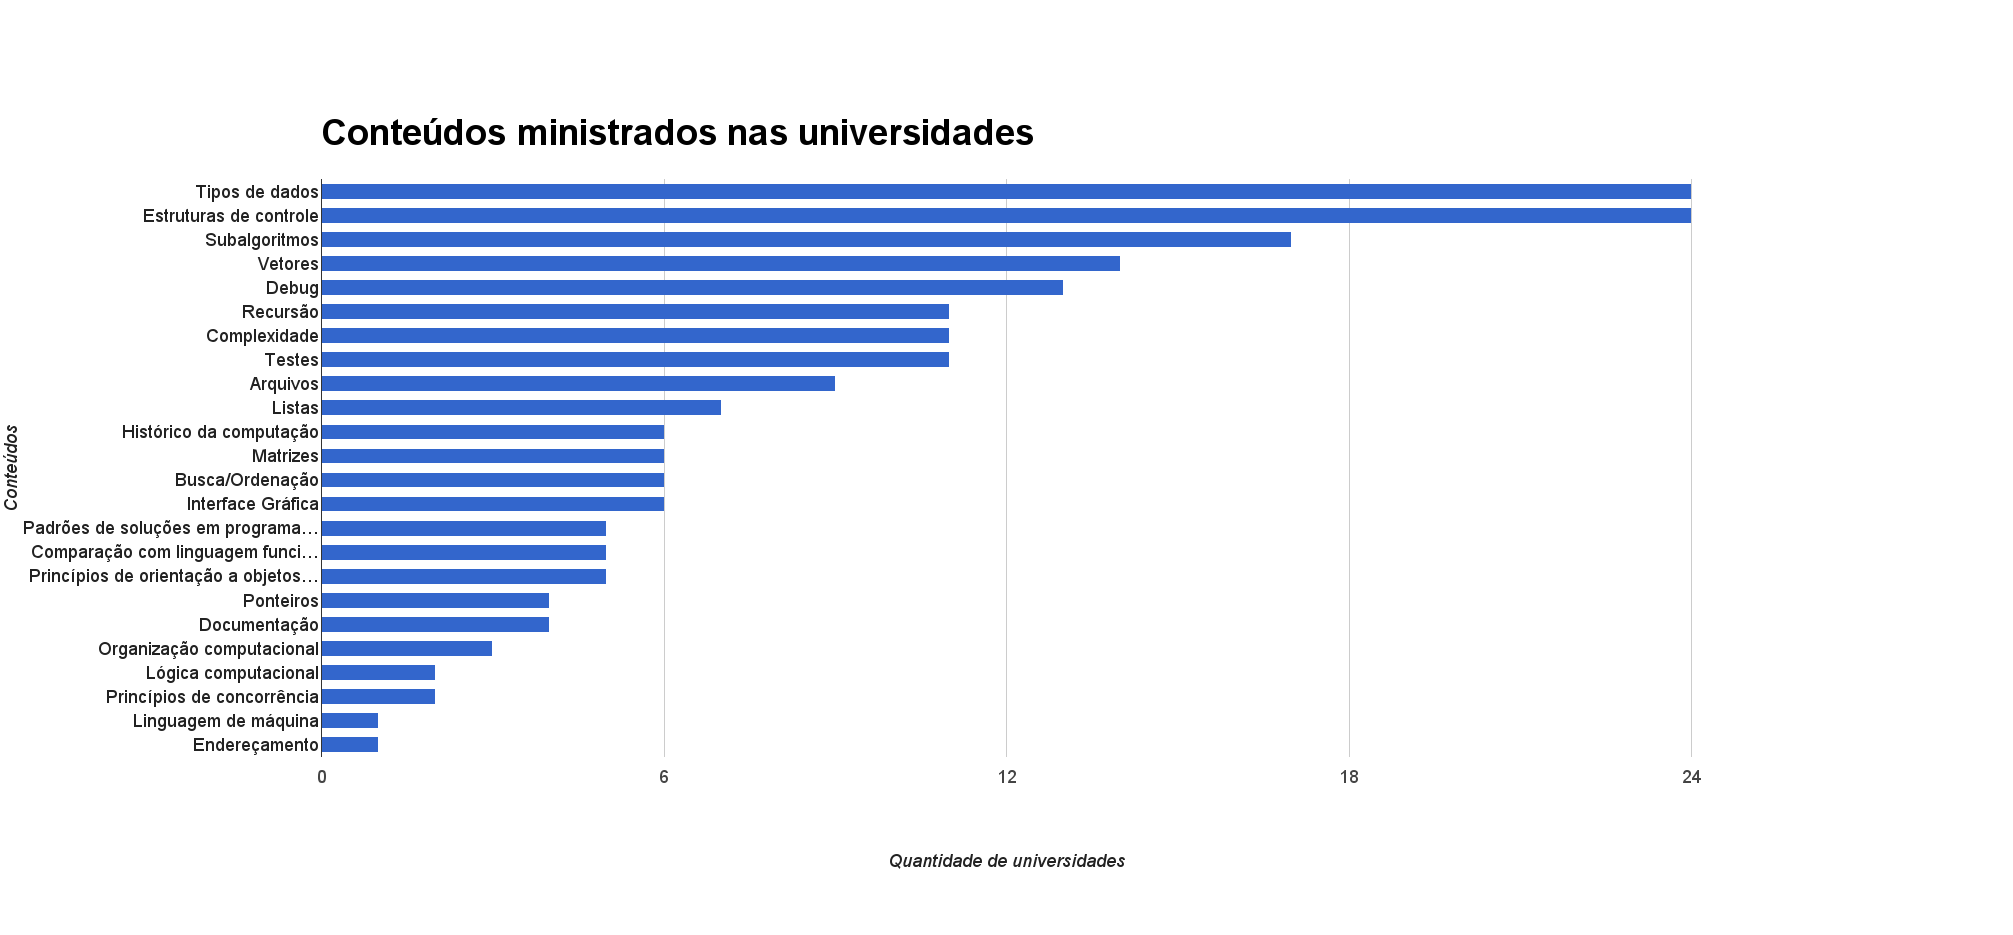
\includegraphics[scale=0.43]{img/universidades}
  \end{center}
  \caption{Conteúdos ministrados em relação a quantidade de universidades que os abordam. }
  \label{fig:conteudos}
\end{sidewaysfigure}

\tabela{Universidades pesquisadas}{tab:universidades}{|p{0.3\textwidth} |p{0.7\textwidth} |}%
  {\hline
  \textbf{Universidade} & \textbf{Curso} \\\hline
  UnB                       & Algoritmos e programação de computadores  \\\hline
  USP                       & MAC0110 - Introdução à Computação  \\\hline
  Unicamp                       & MC102 - Algoritmos e Programação de Computadores  \\\hline
  Massachusetts Institute of Technology (MIT)                       & 6.00 Introduction to Computer Science and Programming   \\\hline
  University of Warteloo                       & CS 137 Programming Principles   \\\hline
  University of Michigan                       & EECS 183. Elementary Programming Concepts    \\\hline
  Vanderbilt University                      & CS 1101 [Formerly CS 101] Programming and Problem Solving    \\\hline
  PUC-Rio                      & Programação para Informática 1    \\\hline
  Hiroshima University                      & Introduction to Computer Programming    \\\hline
  The University of New Mexico                      & CS 105L: Introduction to Computer Programming using Javascript    \\\hline
  Stanford University                      & CS106A: Programming Methodology (Java)    \\\hline
  University of Oxford                      & Imperative Programming    \\\hline
  Carmegie Mellon University                      & 15110  Principles of Computing    \\\hline
  Havard University                      & Introduction to Computer Science Programming in Python (6.0001)    \\\hline
  University of California, Berkeley (UCB)                      & COMPSCI W10 The Beauty and Joy of Computing    \\\hline
  University of Cambridge                      & Paper 1: Foundations of Computer Science    \\\hline
  The Hong Kong University of Science and Technology (HKUST)                      & COMP 1022P        Introduction to Computing with Java    \\\hline
  ETH Zurich (Swiss Federal Institute of Technology)                      & 252-0835-00L         Computer Science I    \\\hline
  Princeton University                      & COS 126 / EGR 126 (QR) General Computer Science    \\\hline
  National University of Singapore (NUS)                      & CS1101S - Programming Methodology    \\\hline
  The University of Hong Kong                      & ENGG1111 Computer Programming and Applications    \\\hline
  The University of Melbourne                      & COMP10001 Foundations of Computing    \\\hline
  Imperial College London                      & CO120.1-Programming I    \\\hline
  University of Toronto                      & CSC108H1: Introduction to Computer Programming    \\\hline
}%

Dentre os tópicos práticos, foram selecionados os seis mais recorrentes para a elaboração de exercícios, os quais são:
 \begin{itemize}
 \item Tipos de dados;
 \item Estruturas de controle;
 \item Subalgoritmos;
 \item Vetores;
 \item Matrizes e;
 \item Recursão.
 \end{itemize}

 Apesar da \playAPC{} poder potencialmente atender a qualquer um dos tópicos da disciplina \acrshort{APC}, no presente trabalho restringiu-se seu uso a estes seis tópicos mais relevantes.

 \newpage

 \subsection{Requisitos} \label{sec:requisitos}

 \subsubsection{Requisitos não-funcionais}
 \begin{enumerate}
 \item Tecnologia usada deve ser a OpenGL;
 \item Linguagem de desenvolvimento deverá ser C++;
 \item As plataformas que deverão ser compatíveis com a biblioteca deverão ser Windows, Linux (baseados em sistemas Debian) e Mac e;
 \item O sistema de referência deverá ser exclusivamente o sistema de coordenadas cartesiano.
 \end{enumerate}

 Devido a tecnologia escolhida ser a OpenGL, é obrigatório para o funcionamento da biblioteca que tenha uma função que inicialize a janela de contexto e outra que renderize o contexto.

 \paragraph{Inicializar janela de contexto}\mbox{}\\

 
\begin{lstlisting}
void AbreJanela(float largura, float altura, const char* titulo)
\end{lstlisting}

A renderização da \playAPC{} utiliza unidades do plano cartesiano, não unidades em \emph{pixel}. Desta forma, todos os cálculos referentes a posicionamento de geometrias não dependem do tamanho da janela em \emph{pixel}, mas sim da posição no plano cartesiano, onde o centro sempre estará no meio da janela.

A função \emph{AbreJanela} inicializa todas as variáveis utilizadas pela biblioteca, e preferencialmente é a chamada antes de qualquer outra função da \playAPC{}. Por padrão, o plano de renderização está limitado de (-100,100) em coordenadas $x,y$ do plano cartesiano. Este valor pode ser alterado utilizando a função \emph{MudaLimitesJanela} antes de chamar \emph{AbreJanela}.
Seu primeiro argumento se refere a largura em \emph{pixels} da janela, o segundo a altura em \emph{pixels} e o terceiro se refere ao nome que a janela terá.

O funcionamento desta função dá-se pela seguinte maneira: dado a largura e altura da janela em \emph{pixels}, é necessário descobrir a proporção desta janela para que o sistema respeite as coordenadas de um plano limitado de $-100$ à $100$ unidades, tanto em largura quanto em altura. Esta proporção é encontrada realizando uma regra de três simples como indica a Equação \ref{eq:proporcao}, sendo $\frac{tam}{2}$ é a menor dimensão da janela em \emph{pixels} dividido por $2$, $100$ é a quantidade de unidades total de um dos lados do plano e $x$ é a quantidade de \emph{pixels} de uma unidade do plano de renderização.

\begin{equation} \label{eq:proporcao}
  \begin{matrix}
    \frac{tam}{2}  & - & 100 \\
    x & - & 1 \\
  \end{matrix}
\end{equation}

Como exemplo, considere o caso particular ilustrado na Figura \ref{fig:prop}. A janela tem $800$ \emph{pixels} de largura e $600$ \emph{pixels} de altura e deseja-se renderizar um ponto no lado mais a direta da janela, com $y = 0$. A Figura \ref{fig:propb} ilustra este resultado.

\figura[!h]{../img/janela_n_quadrada}{Caso quando $largura \neq altura$. A exibição plano cartesiano está limitado de $-100$ unidades à $100$ unidades, tanto em $x$ quanto em $y$, onde $100$ unidades equivalem à $300$ \emph{pixels}, ou $200$ unidades equivalem à $600$ \emph{pixels}}{fig:prop}{width=1.0\textwidth}%

\figura[H]{../img/janela_n_quadradab}{Renderização de um ponto vermelho em $(133, 0)$. O ponto está exagerado para melhor visualização}{fig:propb}{width=1.0\textwidth}%

Queremos, então, que o ponto fique à $400$ \emph{pixels} de distância à partir do centro no eixo $x$. É necessário obter essa posição em unidades do plano cartesiano. Este cálculo é feito com uso da Equação \ref{eq:proporcao_ex}, derivada da Equação \ref{eq:proporcao}, onde $300$ é a distância ao longo do eixo $x$ ou $y$ em \emph{pixels} do centro até a borda do plano cartesiano, $400$ é a posição, também em \emph{pixels}, no eixo $x$ onde se deseja renderizar o ponto e $100$ é a medida em unidades do centro até a borda do plano cartesiano.


 % Para manter a proporção, $200$ unidades do plano de renderização equivalem à $600$ \emph{pixels}, ou $100$ unidades equivalem à $300$ \emph{pixels}, uma vez que a janela é divida em quadrantes positivos e negativos. Suponha que deseja-se renderizar um ponto no canto inferior direito da janela. Como esta coordenada está fora do plano cartesiano renderizado, é necessário utilizar a Equação \ref{eq:proporcao_ex} para calcular sua posição. 

\begin{equation} \label{eq:proporcao_ex}
  \begin{matrix}
    300 &  - & 100 \\
    400 & - & x \\
  \end{matrix}
\end{equation}

Desta forma, encontramos que o valor desejado de $x \cong 133$.

 \paragraph{Renderizar contexto}\mbox{}\\

 
\begin{lstlisting}
void Desenha()
\end{lstlisting}


A função \emph{Desenha} realiza o laço de renderização. Todas as geometrias criadas até esta chamada de função serão renderizadas e permanecerão estáticas, não havendo a possibilidade de posteriores animações.
Para encerrar o laço de renderização, basta fechar a janela clicando no botão de fechar ou apertando a tela \emph{ESC}. Após fechar a janela, todo o contexto da \playAPC{} será encerrado e as áreas de memórias alocadas serão liberadas.

  
\begin{lstlisting}
int Desenha1Frame()
\end{lstlisting}


A função \emph{Desenha1Frame} renderiza pelo menos $\frac{1}{60}$ segundos da cena. Caso o usuário feche a janela ou aperte a tecla ESC, esta função retornará 0 e encerrará o processo de renderização. Caso contrário, retornará 1.

 \subsubsection{Requisitos funcionais para renderização de formas geométricas}
 \begin{enumerate}
 \item O usuário deverá ser capaz de manipular o tipo de dado \emph{ponto}, que possui coordenada $x$ e coordenada $y$;
 \item O usuário deve ser capaz de criar formas geométricas como ponto, reta, polígono, círculo, circunferência, elipse, triângulo, quadrado e retângulo, respeitando definições matemáticas;
 \item O usuário, ao passar um vetor de pontos para uma função específica, deverá conseguir exibir um gráfico;
 \item O usuário deve ser capaz de colorir todas as formas geométricas;
 \item O usuário deve ser capaz de aplicar texturas nas formas geométricas;
 \end{enumerate}

\paragraph{Tipo de dado Ponto}\mbox{}\\

 
\begin{lstlisting} 
struct Ponto{
    float x;
    float y;
}
\end{lstlisting}


Ponto é uma estrutura do tipo float com dois membros, \emph{x} e \emph{y}, os quais devem ser utilizados como coordenadas do plano cartesiano 2D. Esta estrutura possui sobrecarga para os seguintes operadores =, +, -, +=, -=, == e !=.
\begin{itemize}
  \item =
    \begin{lstlisting}
    Ponto p1, p2;
    (...)

    p1 = p2;
    \end{lstlisting}
   \item + (ou -)
    \begin{lstlisting}
    Ponto p1, p2, p3;
    (...)

    p1 = p2 + p3;
    \end{lstlisting} 
     \item += (ou -=)
    \begin{lstlisting}
    Ponto p1, p2;
    (...)

    p1 += p2;
    \end{lstlisting}

     \item == (ou !=)
    \begin{lstlisting}
    Ponto p1, p2;
    (...)

    if(p1 == p2){
      (...)
    }
    \end{lstlisting}
\end{itemize}

\paragraph{Forma geométrica Ponto}\mbox{}\\

 
\begin{lstlisting}
int CriaPonto(Ponto p)
\end{lstlisting}


A função \emph{CriaPonto} cria uma geometria do tipo \emph{PONTO}, retornando um índice deste tipo de geometria. Seu único argumento é uma variável do tipo Ponto. Uma geometria do tipo \emph{PONTO} é renderizada como um \emph{pixel}.

\paragraph{Forma geométrica Reta}\mbox{}\\

 
\begin{lstlisting} 
int CriaReta(Ponto p1, Ponto p2)
\end{lstlisting}


A função \emph{CriaReta} cria uma geometria do tipo \emph{RETA}, retornando um índice deste tipo de geometria. Seu primeiro e segundo argumento são duas variáveis do tipo Ponto.

\paragraph{Forma geométrica Polígono}\mbox{}\\

 
\begin{lstlisting}
int CriaPoligono(short int qtd, ...)
\end{lstlisting}


A função \emph{CriaPoligono}, cria uma geometria do tipo \emph{POLIGONO}, retornando um índice deste tipo de geometria. Seu primeiro argumento é a quantidade de pontos que serão passados para esta função, e os seguintes argumentos serão os pontos propriamente ditos. Note que a \playAPC{} é limitada no aspecto que esta função só consegue renderizar figuras convexas por conta da OpenGL. Caso haja a necessidade de criação de figuras não-convexas, será necessário \emph{"quebrar"} a geometria não-convexa em duas ou mais geometrias convexas.

 
\begin{lstlisting}
int CriaPoligonoVetor(short int index, Ponto *p)
\end{lstlisting}


A função \emph{CriaPoligonoVetor} cria e retorna o mesmo tipo de geometria que a \emph{CriaPoligono}. Entretanto, seu diferencial são seus argumentos: seu primeiro argumento é o tamanho do vetor e o segundo argumento o vetor propriamente dito.

\paragraph{Forma geométrica Círculo}\mbox{}\\

 
\begin{lstlisting} 
int CriaCirculo(float raio, Ponto meio)
\end{lstlisting}


A função \emph{CriaCirculo}, cria uma geometria do tipo \emph{CIRCULO}, retornando um índice deste tipo de geometria. Seu primeiro argumento é o tamanho do raio e o segundo argumento é onde estará centrado o círculo.

\paragraph{Forma geométrica Circunferência}\mbox{}\\

 
\begin{lstlisting}
int CriaCircunferencia(float raio, Ponto meio)
\end{lstlisting}


A função \emph{CriaCircunferencia}, cria uma geometria do tipo \emph{CIRCUNFERENCIA}, retornando um índice deste tipo de geometria. Seu primeiro argumento é o tamanho do raio e o segundo argumento é onde estará centrada a circunferência.

\paragraph{Forma geométrica Elipse}\mbox{}\\

 
\begin{lstlisting}
int CriaElipse(float a, float b, Ponto meio)
\end{lstlisting}


A função \emph{CriaElipse}, cria uma geometria do tipo \emph{ELIPSE}, retornando um índice deste tipo de geometria. Seu primeiro argumento é a metade do maior eixo da elipse, o segundo é a metade do menor eixo da elipse e o terceiro argumento se refere onde a elipse estará centrada.

\paragraph{Forma geométrica Triângulo}\mbox{}\\

 
\begin{lstlisting}
int CriaTriangulo(float base, float altura, Ponto cantoesq)
\end{lstlisting}


A função \emph{CriaTriangulo} cria uma geometria do tipo \emph{TRIANGULO}, retornando um índice deste tipo de geometria. Seu primeiro argumento é a base do triângulo, o segundo a altura não-negativa dele e o último é onde ficará localizado o ponto esquerdo inferior da geometria.

\paragraph{Forma geométrica Quadrado}\mbox{}\\

 
\begin{lstlisting}
int CriaQuadrado(float lado, Ponto cantoesq)
\end{lstlisting}


A função \emph{CriaQuadrado} cria uma geometria do tipo \emph{QUADRADO}, retornando um índice deste tipo de geometria. Seu primeiro argumento é o tamanho do lado do quadrado e o segundo argumento é onde ficará localizado o ponto esquerdo inferior da geometria.

\paragraph{Forma geométrica Retângulo}\mbox{}\\

 
\begin{lstlisting}
int CriaRetangulo(float base, float altura, Ponto cantoesq)
\end{lstlisting}


A função \emph{CriaRetangulo} cria uma geometria do tipo \emph{RETANGULO}, retornando um índice deste tipo de geometria. Seu primeiro argumento é a base do retângulo, o segundo a altura não-negativa dele e o último é onde ficará localizado o ponto esquerdo inferior da geometria.

\paragraph{Renderização de gráficos}\mbox{}\\
 
\begin{lstlisting}
int CriaGrafico(short int index, Ponto *p, short int verTipo)
\end{lstlisting}


A função \emph{CriaGrafico} cria uma geometria do tipo \emph{GRAFICO}, retornando um índice deste tipo de geometria. A partir de um vetor de pontos \emph{p} de tamanho \emph{index}, esta função cria uma sequência de retas que ligam cada ponto definido pelo vetor. O seu terceiro argumento, \emph{verTipo}, se refere o modo de visualização do gráfico, recebendo os parâmetros descritos na Tabela \ref{tab:CriaGrafico}.


\tabela{Valor de \emph{verTipo} da função \emph{CriaGrafico}}{tab:CriaGrafico}{|p{0.3\textwidth} |p{0.7\textwidth} |}%
  {\hline
  \textbf{Valor} & \textbf{Descrição} \\\hline
  0                       & Não redimensiona a tela  \\\hline
  1                       & Redimensiona a tela a fim de comportar toda a função dentro da janela de renderização  \\\hline
  2                       & Redimensiona a tela a fim de comportar toda a função dentro da janela de rendedização sem interferir na escala de ambos os eixos \\\hline
}%

\paragraph{Colorir formas geométricas}\mbox{}\\
A função \emph{Pintar} pode ser utilizada de duas formas diferentes.

 
\begin{lstlisting}
void Pintar(int red, int green, int blue) 
\end{lstlisting}


A última geometria criada receberá a cor definida utilizando o sistema de cores RGB. O primeiro argumento é o componente vermelho, o segundo o componente verde e o terceiro o componente azul, todos variando de $0$ à $255$.

 
\begin{lstlisting} 
void Pintar(int red, int green, int blue, 
	  geometrias_validas nome, int index)
\end{lstlisting}


Apenas a geometria do tipo \emph{nome} com índice definida por \emph{index} será pintada com as cores especificadas pelos valores \emph{red, green e blue}. O quarto argumento é o tipo de geometria, podendo variar de acordo com a função com prefixo \emph{Cria} utilizado, o quinto argumento é o retorno das funções com prefixo \emph{Cria}. 
De forma resumida, o argumento \emph{nome}, do tipo \emph{geometrias\_validas}, pode receber os valores descritos na Tabela ~\ref{tab:PintarM2}.


\tabela{Valor de \emph{nome} da função \emph{Pintar} e \emph{AssociaImagem}}{tab:PintarM2}{|p{0.3\textwidth} |p{0.7\textwidth} |}%
  {\hline
  \textbf{Valor} & \textbf{Retorno da função} \\\hline
  CIRCULO                       & CriaCirculo  \\\hline
  QUADRADO                       & CriaQuadrado  \\\hline
  CIRCUNFERENCIA                       & CriaCircunferencia \\\hline
  RETANGULO                       & CriaRetangulo \\\hline
  ELIPSE                       & CriaElipse \\\hline
  GRAFICO                       & CriaGrafico \\\hline
  PONTO                       & CriaPonto \\\hline
  RETA                       & CriaReta \\\hline
  POLIGONO                       & CriaPoligono e CriaPoligonoVetor \\\hline
  TRIANGULO                       & CriaTriangulo \\\hline
}%

\newpage
\paragraph{Mostrar imagens em formas geométricas}\mbox{}\\

\begin{lstlisting}
int AbreImagem(const char *src)
\end{lstlisting}

A função \emph{AbreImagem} abre uma imagem e a deixa-a pronta para ser vinculada a alguma geometria. Seu primeiro parâmetro é o caminho da imagem e ela retorna o índice de textura para ser vinculado.

Para vincular uma imagem a uma geometria, existem duas formas de usar a função \emph{AssociaImagem}
\begin{lstlisting}
void AssociaImagem(int textura)
\end{lstlisting}
A última geometria criada receberá a imagem associada àquela textura. Seu único argumento é o índice de textura, retorno da função \emph{AbreImagem}.


\begin{lstlisting}
void AssociaImagem(int textura, geometrias_validas nome, int index)
\end{lstlisting}
Apenas a geometria do tipo \emph{nome} com índice definida por \emph{index} receberá a imagem associada àquela textura. O segundo argumento é o tipo de geometria, podendo variar de acordo com a função com prefixo \emph{Cria} utilizado, o terceiro argumento é o retorno das funções com prefixo \emph{Cria}. 
O argumento \emph{nome}, do tipo \emph{geometrias\_validas}, pode receber os valores descritos na Tabela ~\ref{tab:PintarM2}.

 \subsubsection{Requisitos funcionais para animação}
 \begin{enumerate}
 \item O usuário deve ser capaz de realizar animações dentro de um laço de repetição;
 \item O usuário deverá ser capaz de movimentar, girar e redimensionar uma ou mais geometrias e;
 \item O usuário deverá ser capaz de limpar cenas ou geometrias criadas;
 \end{enumerate}

 \paragraph{Renderizar cena dentro de um laço de repetição}\mbox{}\\

 Utilizando a função \emph{Desenha1Frame} dentro de um laço de repetição, ela irá renderizar $\frac{1}{60}$ segundos da cena. Sendo assim, pode ter definições de novas geometrias ou transformações antes ou depois da função ser chamada.

  \paragraph{Agrupando mais de uma geometria}\mbox{}\\

Para a animação de um conjunto de geometrias, se faz necessário a criação de um grupo.

\begin{lstlisting} 
int CriaGrupo ( )
\end{lstlisting}
A função \emph{CriaGrupo} agrupa todo um conjunto de geometrias, associando todas a um único índice, em um único conjunto. Desta forma, é possível transformar um conjunto de geometrias de forma independente, apenas referenciando o índice do grupo. Todas as geometrias criadas após a chamada desta função pertencerão ao mesmo grupo.

Caso o programa não utilize esta função para criação de um grupo, todas as geometrias definidas pertencerão ao mesmo grupo.

\paragraph{Movimentação de uma ou mais geometrias}\mbox{}\\
Há duas maneiras de utilizar a função \emph{Move}: ou ela translada o último grupo criado ou ela translada um grupo específico. Independente de qual grupo que sofrerá a ação de movimentar, todas as geometrias do grupo serão transladadas até que o ponto de referência da primeira geometria deste grupo esteja no novo ponto desejado.

\begin{lstlisting}
void Move( Ponto p)
\end{lstlisting}
Seu argumento é o ponto no plano cartesiano que se deseja mover as geometrias, onde ele irá movimentar o último grupo definido. 

\begin{lstlisting}
void Move(Ponto p, int index)
\end{lstlisting}
Seu primeiro argumento é o ponto no plano cartesiano que se deseja mover as geometrias e o segundo argumento o índice do grupo para ser movimentado, índice criado pela função \emph{CriaGrupo}. 

\paragraph{Rotação de uma ou mais geometrias}\mbox{}\\
Há duas maneiras de utilizar a função \emph{Gira}: ou ela rotaciona o último grupo criado ou ela rotaciona um grupo específico. Independente de qual grupo que sofrerá a ação de girar, todas as geometrias do grupo serão rotacionados até que o ponto de referência da primeira geometria deste grupo esteja no novo ponto desejado.

\begin{lstlisting}
void Gira( float theta )
\end{lstlisting}

Seu argumento é o ângulo em graus que o último grupo criado deverá ser rotacionada. O grupo irá rotacionar em relação ao plano cartesiano, não ao seu próprio eixo. 

\begin{lstlisting}
void Gira( float theta , int index )
\end{lstlisting}
Seu primeiro argumento é o ângulo em graus que o grupo com o índice \emph{index} será rotacionado. O grupo irá rotacionar em relação ao plano cartesiano, não ao seu próprio eixo. 

\paragraph{Redimensionar uma ou mais geometrias}\mbox{}\\
Há duas maneiras de utilizar a função \emph{Redimensiona}: ou ela redimensiona o último grupo criado ou ela redimensiona um grupo específico. Independente de qual grupo que sofrerá a ação de redimensionar, todas as geometrias do grupo serão redimensionadas com a fator passado em $x$ e em $y$.

\begin{lstlisting}
void Redimensiona(float x, float y)
\end{lstlisting}

Seu primeiro argumento é o fator em $x$ e seu segundo argumento é o fator em $y$ de distorção que as geometrias do último grupo criado sofrerão.

\begin{lstlisting}
void Redimensiona(float x, float y, int index)
\end{lstlisting}
Seu primeiro argumento é o fator em $x$, seu segundo argumento é o fator em $y$ e seu terceiro argumento é o grupo que as geometrias serão distorcidas.

\paragraph{Limpar a cena}\mbox{}\\

\begin{lstlisting}
void ApagaGrupo(int index)
\end{lstlisting}
A função \emph{ApagaGrupo} destrói todas as geometrias do grupo \emph{index}. Seu argumento é o grupo que deverá ser apagado, que é retorno da função \emph{CriaGrupo}.

\begin{lstlisting}
void LimpaDesenho()
\end{lstlisting}
Limpa toda a cena, destruindo grupos e geometrias. Porém, não altera cor de fundo nem limites do eixo de coordenadas.

 \subsubsection{Requisitos funcionais para entrada de mouse e teclado}
 \begin{enumerate}
 \item O usuário deve informar uma tecla ou botão do mouse para uma função e esta deve retornar se ela foi pressionada e;
 \item O usuário deve ser informado qual a posição do mouse em relação ao plano cartesiano;
 \end{enumerate}

 \paragraph{Entrada de teclado}\mbox{}\\
\begin{lstlisting}
int ApertouTecla(int tecla)
\end{lstlisting}
A função \emph{ApertouTecla} retorna $1$ se o usuário pressionou ao menos uma vez a tecla $tecla$ e retorna $0$ caso contrário. Seu argumento é uma das possíveis teclas do teclado, listados na Tabela \ref{tab:teclas}.

\tabela{Teclas reconhecidas pela \playAPC}{tab:teclas}{|p{0.4\textwidth} |p{0.6\textwidth} |}%
  {\hline
  \textbf{Valor} & \textbf{Descrição} \\\hline
    '$n$'  & Teclas alfanuméricas ($n \in (0..9)$ ou $n \in (A..Z)$)  \\\hline
    GLFW\_KEY\_SPACE  & Espaço \\\hline
    GLFW\_KEY\_ESC  & Escape \\\hline
    GLFW\_KEY\_F$n$  & Function key ($n \in (0..25)$) \\\hline
    GLFW\_KEY\_LEFT  & Seta para esquerda \\\hline
    GLFW\_KEY\_UP  & Seta para cima \\\hline
    GLFW\_KEY\_DOWN  & Seta para baixo \\\hline
    GLFW\_KEY\_RIGHT  & Seta para direita \\\hline
    GLFW\_KEY\_LCONTROL  & Control esquerdo \\\hline
    GLFW\_KEY\_RCONTROL  & Control direito \\\hline
    GLFW\_KEY\_LALT  & Alt esquerdo \\\hline
    GLFW\_KEY\_RALT  & Alt direito \\\hline
    GLFW\_KEY\_TAB  & Tabulador \\\hline
    GLFW\_KEY\_ENTER  & Enter \\\hline
    GLFW\_KEY\_BACKSPACE  & Backspace \\\hline
    GLFW\_KEY\_INSERT  & Insert \\\hline
    GLFW\_KEY\_DEL  & Delete \\\hline
    GLFW\_KEY\_PAGEUP  & Page up \\\hline
    GLFW\_KEY\_PAGEDOWN  & Page down \\\hline
    GLFW\_KEY\_HOME  & Home \\\hline
    GLFW\_KEY\_END  & End \\\hline
    GLFW\_KEY\_KP\_$n$  & Teclas numéricas do keypad ($n \in (0..9)$)\\\hline
    GLFW\_KEY\_KP\_DIVIDE  & Tecla dividir do keypad ( $\div $)\\\hline
    GLFW\_KEY\_KP\_MULTIPLY  & Tecla multiplicar do keypad ( $\times$ )\\\hline
    GLFW\_KEY\_KP\_SUBTRACT  & Tecla subtrair do keypad ( - )\\\hline
    GLFW\_KEY\_KP\_ADD  & Tecla adição do keypad ( + )\\\hline
    GLFW\_KEY\_KP\_EQUAL  & Tecla igual do keypad ( = )\\\hline
    GLFW\_KEY\_KP\_NUMLOCK  & Tecla Numlock do keypad ( = )\\\hline
    GLFW\_KEY\_CAPS\_LOCK  & Caps lock\\\hline
    GLFW\_KEY\_SCROLL\_LOCK  & Scroll lock\\\hline
    GLFW\_KEY\_PAUSE  & Pause\\\hline
    GLFW\_KEY\_MENU  & Menu\\\hline
}%

\begin{lstlisting}
int RetornaTecla()
\end{lstlisting}
Ao usuário digitar qualquer tecla reconhecível pela \playAPC{}, esta função retorna qual tecla foi essa, listada na Tabela \ref{tab:teclas}.

 \paragraph{Entrada de mouse}\mbox{}\\

\begin{lstlisting}
int ApertouBotaoMouse(int bt)
\end{lstlisting}
A função \emph{ApertouBotaoMouse} retorna $1$ se o usuário pressionou ao menos uma vez o botão $bt$ e retorna $0$ caso contrário. Seu argumento é um dos possíveis botões do mouse, listados na Tabela \ref{tab:botoes}.

\tabela{Botões de mouse reconhecidos pela \playAPC}{tab:botoes}{|p{0.4\textwidth} |p{0.6\textwidth} |}%
  {\hline
  \textbf{Valor} & \textbf{Descrição} \\\hline
GLFW\_MOUSE\_BUTTON\_$n$  & Botões possíveis do mouse ($n \in (0..8)$ )  \\\hline
    GLFW\_MOUSE\_BUTTON\_LEFT  & Botão esquerdo ($n \gets 1)$\\\hline
    GLFW\_MOUSE\_BUTTON\_RIGHT  & Botão direito ($n \gets 2)$\\\hline
    GLFW\_MOUSE\_BUTTON\_MIDDLE  & Botão do meio ($n \gets 3)$\\\hline
}%

\begin{lstlisting}
int RetornaBotaoMouse()
\end{lstlisting}
Ao usuário apertar qualquer botão reconhecível pela \playAPC{}, esta função retorna qual botão foi esse, listado na Tabela \ref{tab:botoes}.

\begin{lstlisting} 
void PosicaoMouse(int *x, int *y)
\end{lstlisting}
A função \emph{PosicaoMouse} retorna para $x$ e $y$ atual posição do mouse em relação ao plano cartesiano. Se a janela de contexto não estiver em foco ou se o mouse não estiver sobre a janela, a função irá retornará a última posição registrada. No começo da execução, é necessário que as variáveis $x$ e $y$ estejam inicializadas. Seus argumentos são as variáveis $x$ e $y$ que receberão a posição atual do mouse.

 \subsubsection{Requisitos funcionais para outros tipos de funções}
 \begin{enumerate}
 \item O usuário deve ser capaz de colorir o fundo da janela
 \item O usuário deve ter noção dos limites do plano cartesiano;
 \item O usuário deve ser capaz de alterar os limites de renderização;
 \item O usuário deve ser capaz de, dado uma imagem, extrair os componentes RGB da mesma na forma de uma matriz R, G e B e;
 \item O usuário deve ser capaz de aumentar a espessura da borda de uma geometria;
 \end{enumerate}

  \paragraph{Colorir plano de fundo da janela}\mbox{}\\

  \begin{lstlisting}
void PintaFundo(int red, int green, int blue)
\end{lstlisting}
Colore o plano de fundo da janela com a cor passada pelos parâmetros $red$, $green$ e $blue$, que respeitam o sistemas de cores RGB. Seu primeiro argumento é o componente vermelho, o segundo é o verde e o terceiro o azul.

 \paragraph{Plano de renderização}\mbox{}\\

  \begin{lstlisting}
void MudaLimitesJanela(int limite)
\end{lstlisting}
Esta é a única função da \playAPC{} que, se for utilizada, deve ser chamada antes da função \emph{AbreJanela}. Ela altera os limites das coordenadas da playAPC. Caso esta função não seja chamada, os limites são por padrão de $-100$ à $100$, tanto no eixo horizontal quanto no eixo vertical. Seu argumento é o limite positivo de até onde a janela de visualização deve renderizar, que será utilizado tanto no eixo vertical quanto no original indo de $-limite$ até $limite$.

 \begin{lstlisting}
void MostraPlanoCartesiano(int intervalo)
\end{lstlisting}
Exibe linhas das coordenadas da \playAPC{} de $-100$ à $100$ no eixo horizontal e vertical, caso os limites não sejam alterados. Seu centro é localizado em $(0,0)$ e é identificado pelas linhas pretas. As linhas cinzas indentificam o intervalo das coordenadas. Seu argumento são os espaçamentos entre as linhas em cinza.
Esta função serve para auxiliar o usuário a identificar onde serão renderizadas suas geometrias.

 \paragraph{Componentes RGB de uma imagem}\mbox{}\\
  \begin{lstlisting}
void ExtraiRGBdeBMP(const char *imagepath, int largura, int altura, 
  int (&R)[tam_x][tam_y], int (&G)[tam_x][tam_y], int (&B)[tam_x][tam_y])
\end{lstlisting}
Dado uma imagem BMP de 24 bits, a função lê a imagem e extrai os componentes vermelho, verde e azul dela. Seu primeiro argumento é o caminho da imagem, seu segundo e terceiro argumentos são a largura e altura da imagem, seu quarto, quinto e sexto argumento são as matrizes que irão receber os componentes vermelho, verde e azul, respectivamente. As matrizes precisarão ter necessariamente a quantidade de linhas e colunas maior ou igual aos parâmetros $largura$ e $altura$.

\paragraph{Alterar espessura da borda}\mbox{}\\
 \begin{lstlisting}
void Grafite(int espessura)
\end{lstlisting}
Rasterização, em computação gráfica, é o processo que determina quais \emph{pixels} serão utilizados para a renderização de uma geometria.

A função \emph{Grafite} aumenta a quantidade de linhas de rasterização da última geometria criada, variando de 1 a $\infty$. Seu parâmetro é quanto se deseja aumentar as linhas. Por padrão, todas as geometrias começam com esta linha igual a 1. Esta função pode ser usada para deixar mais visível geometrias do tipo \emph{PONTO}, que possuem 1 \emph{pixel} de tamanho.


















\subsection{Arquitetura da biblioteca}
A arquitetura em camadas foi escolhida por conta de sua manutenibilidade, apesar que, dependendo do caso, a arquitetura acaba resultando em uma queda de desempenho por ter camadas que chamam um método de uma camada anterior. Um exemplo é a função \emph{PintarFundo}, a qual está na camada mais superior, a interface da \playAPC{}, que chama um método da camada \emph{Evento} que chama uma única função da Opengl, a \emph{glClear}.

Porém, suponha que fosse necessário mudar a API GLFW 2.7 para a GLFW 3.0, ou mudar para a biblioteca GLUT. Para isso, bastaria apenas modificar a classe \emph{OpenglBase}, mantendo os métodos ou adicionando novos, se fosse o caso. 

A Fig.~\ref{fig:arq} ilustra esta arquitetura é utilizada e como cada camada se comunica.

\begin{figure}[ht!]
\centering  %\includegraphics[scale=0.5]{Arquitetura_PlayCB}
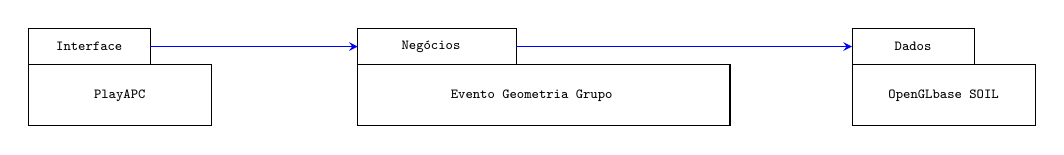
\begin{tikzpicture}[>=stealth,scale=1.55]
\draw (0,.5) rectangle (1,.8); \node at (.5,.65) 
        {\tiny\texttt{\textbf{Interface}}};
\draw (0,0) rectangle (1.5,.5);
\node at (.75,.25) {\tiny\texttt{PlayAPC}};

\draw (2.7,.5) rectangle (4,.8); \node at (3.3,.65) 
        {\tiny\texttt{\textbf{Negócios}}};
\draw (2.7,0) rectangle (5.75,.5);
\node at (4.125,.25) {\tiny\texttt{Evento Geometria Grupo}};

\draw (6.75,.5) rectangle (7.75,.8); \node at (7.25,.65) 
        {\tiny\texttt{\textbf{Dados}}};
\draw (6.75,0) rectangle (8.25,.5);
\node at (7.5,.25) {\tiny\texttt{OpenGLbase SOIL}};

\draw[->,blue] (1,.65) -- (2.7,.65);
\draw[->,blue] (4,.65) -- (6.75,.65);
\end{tikzpicture}
\caption{Organização da arquitetura da \playAPC.}
\label{fig:arq}
\end{figure}

\begin{itemize}
\item A camada de interface é a comunicação entre o usuário e a biblioteca gráfica,
que trata desde  a criação de objetos a serem exibidos  na tela até ao
laço de renderização, todos estruturados de forma sequencial, em que o
usuário  possa  escrever  um  programa  sem a  necessidade  de  ter  o
conhecimento de orientação a objeto. Esta camada abrange o seguinte código fonte e o arquivo de cabeçalho, ambos de mesmo nome:
  \begin{itemize}
    \item playapc
  \end{itemize}

\item A camada de  dados é responsável pela manipulação  da biblioteca GLFW,
responsável  pela  criação de  janelas  com  o  contexto da  OpenGL  e
gerencia  os eventos  para  renderização, sendo  chamada somente  pela
camada de negócios. É também nesta camada que se encontra bibliotecas de terceiros que foram incorporados à \playAPC{}. Ela possui os seguintes arquivos:
  \begin{itemize}
    \item OpenglBase
    \item SOIL
  \end{itemize}

\item A  camada  de  negócios  é  a camada  que  constrói  objetos,  realiza
transformações  algébricas  e   gerencia  chamadas  para  controle  de
renderização.  Grande parte do código fonte da \playAPC{} se concentra nessa camada, pois esta abrange os seguintes códigos fontes e seus respectivos arquivos de cabeçalhos:
  \begin{itemize}
    \item Grupo
    \item Evento
    \item PlanoCartesiano
    \item Geometria
      \begin{itemize}
        \item Circulo
        \item Circunferencia
        \item Elipse
        \item Poligono
        \item Pontinho
        \item Reta
        \item Retangulo
        \item Triangulo
        \item Grafico
      \end{itemize}
  \end{itemize}
\end{itemize}


Toda a camada de interface da \playAPC{} utiliza a metodologia de encapsulamento para simplificar o processo de criação de geometrias e sua renderização, tendo o melhor exemplo nesta camada a função \emph{Desenha}, que esconde a informação de que esta função é responsável pelo laço de renderização.

\begin{figure}[h!]
  \begin{center}
    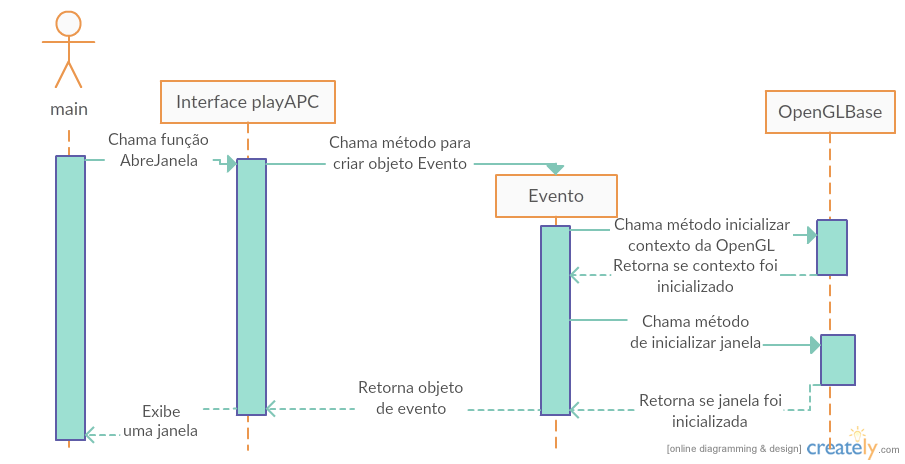
\includegraphics[width=1.0\textwidth]{img/Sequencia_playcb}
  \end{center}
  \caption{Diagrama de Sequência da função \emph{AbreJanela}.}
  \label{fig:sequencia}
\end{figure}

Como exemplo particular, ilustrado na Figura \ref{fig:sequencia}, para o funcionamento desta chamada de função \emph{AbreJanela}, a interface da \playAPC{} cria um objeto do tipo \emph{Evento}, sendo esta classe responsável por gerenciar todos os eventos de entrada e renderização. Note que não há a necessidade de saber como é implementado este objeto para a main, tornando o próprio objeto \emph{Evento} independente de código, uma vez que sua funcionalidade foi abstraída para somente devolver ao usuário uma janela de contexto.


A \playAPC{} utiliza o método Herança com a classe Geometria, que possui métodos e atributos em comum com as subclasses Círculo, Circunferência, Elipse, Polígono, Reta, Retângulo, Ponto, Gráfico e Triângulo.
\begin{lstlisting}%
[caption={Descrição da classe Geometria.}, label=geometria,
emph={AbreJanela,PintarFundo,Ponto,CriaCircunferencia,CriaCirculo,CriaGrupo,%
Pintar,Grafite,Move,Desenha,Desenha1Frame}, style=tuto]
class Geometria{
    protected:
        GLfloat red, green, blue;
        GLfloat grafite;
        Geometria *prox;
        GLuint textura;
    public:
        ///Métodos virtuais
        virtual void RenderizaPontos() = 0; //Método para desenhar as geometrias, com glBegin() e glEnd()
        virtual Ponto CalculaDeslocamento(Ponto p) = 0;

        ///Métodos em comum de todas as geometrias
        void Cor(GLfloat red = 0, GLfloat green = 0, GLfloat blue = 0); //Define cores
        void Grafite(GLfloat grafite = 1.0); //Define grossura da borda
        void Agrupa(Geometria *prox); //Cria lista de geometrias
        void Desagrupa(Geometria **atual, Geometria *primeiro); //Tira da lista algum elemento
        Geometria *getProx(); //Pega o próximo elemento da lista
        GLuint getTextura(); //Retorna área alocada para textura
        void setTextura(GLuint data); //Seta área alocada para textura
};
\end{lstlisting}

As classes referentes às geometrias que podem ser criadas com a \playAPC{} se diferenciam no método \emph{RenderizaPontos} e no método de \emph{CalculaDeslocamento}, visto que estes métodos são virtuais. Para o método de \emph{RenderizaPontos}, cada um dos herdeiros utilizam a função da OpenGL \emph{glBegin()} e \emph{glEnd()} passando diferentes argumentos dependendo do tipo de geometria.
\begin{itemize}
  \item A classe \emph{Pontinho} é criada a partir de um único \emph{Ponto p} passado pelo usuário e utiliza como argumento para \emph{glBegin()} o \emph{GL\_POINTS}.
  \item A classe \emph{Reta} é criada a partir de dois pontos \emph{Ponto p1} e \emph{Ponto p2} passado pelo usuário e utiliza como argumento para \emph{glBegin()} o \emph{GL\_LINES}.
  \item A classe \emph{Poligono} é criada a partir de $n$ pontos, agrupados em uma lista, passado pelo usuário e utiliza como argumento para \emph{glBegin()} o \emph{GL\_POLYGON}.
  \item A classe \emph{Triangulo} é criada a partir de um único ponto \emph{Ponto p} de referência, que é o ponto do canto esquerdo inferior, um valor para a base e um valor para a altura passados pelo usuário e utiliza como argumento para \emph{glBegin()} o \emph{GL\_TRIANGLES}.
  \item A classe \emph{Retangulo}, que é a mesma utilizada para criar quadrados com \emph{CriaQuadrado}, é criada a partir de um único ponto \emph{Ponto p} de referência, que é o ponto do canto esquerdo inferior, um valor para a base e um valor para a altura passados pelo usuário e utiliza como argumento para \emph{glBegin()} o \emph{GL\_QUADS}.
  \item A classe \emph{Circulo} é criada a partir de um único ponto \emph{Ponto p} de referência, que é o ponto do centro do círculo e um valor o raio passados pelo usuário e utiliza como argumento para \emph{glBegin()} o \emph{GL\_TRIANGLE\_FAN}. 
  \item A classe \emph{Circunferencia} é criada a partir de um único ponto \emph{Ponto p} de referência, que é o ponto do centro da circunferência e um valor o raio passados pelo usuário e utiliza como argumento para \emph{glBegin()} o \emph{GL\_LINE\_LOOP}. 
  \item A classe \emph{Elipse} é criada a partir de um único ponto \emph{Ponto p} de referência, que é o ponto do centro da elipse, e dois valores que correspondem a metade do lado menor e do lado maior passados pelo usuário e utiliza como argumento para \emph{glBegin()} o \emph{GL\_TRIANGLE\_FAN}.
  \item A classe \emph{Grafico} é criada a partir de $n$ pontos passados pelo vetor \emph{Ponto p*} passado pelo usuário e utiliza como argumento para \emph{glBegin()} o \emph{GL\_LINES}. 
\end{itemize}
O método \emph{CalculaDeslocamento} é um método que, para um ponto $p$ passado como argumento deste método, cada herdeiro calcula a distância que este ponto está em relação ao seu ponto de referência, seja ele o ponto esquerdo, o ponto central ou até mesmo o primeiro ponto que foi passado como argumento na construção de um objeto dele.






















\section{Apresentação da biblioteca} \label{sec:apresentacao}
Para a apresentação da biblioteca, vamos apresentar o clássico problema da Torre de Hanói. Para melhor visualização do problema, a quantidade de discos foi limitada para 5. A Listagem \ref{lst:hanoi_1} apresenta um código em C, com saída textual, com uma das possíveis soluções da torre de Hanói.

\figura[H]{../img/hanoi_1}{Resolução da torre de Hanói para 3 discos}{fig:hanoi1}{width=0.5\textwidth}%
\lstinputlisting[style=code, label=lst:hanoi_1, caption=Código fonte da Torre de Hanói.]{cpp/hanoi_1.cpp}

\subsection{Criação da janela de contexto da \playAPC}
A primeira instrução necessária para usar a \playAPC{}, depois de ter instalado e linkado a biblioteca, é incluir o seu header no código do programa.

 \begin{lstlisting}[caption={Incluir \playAPC{} no código.}, style=tuto] 
#include <stdio.h>
#include <playAPC/playapc.h>
\end{lstlisting}

Agora podemos criar uma janela de contexto com a função \emph{AbreJanela}. Também podemos pintar o fundo desta janela de branco e exibir nosso plano de renderização, o plano cartesiano.
 \begin{lstlisting}[caption={Abrir uma janela branca, mostrando o plano cartesiano.}, style=tuto] 
 (...)
    do{
        printf("\nDigite uma quantidade de discos menor ou igual a 5: ");
        scanf("%d", &numDiscos);
    }while(numDiscos > 5 || numDiscos <= 0);
    
    AbreJanela(400, 400, "Torre de Hanoi");
    PintarFundo(255, 255, 255);
    MostraPlanoCartesiano(10);
(...)
\end{lstlisting}

Ao final da execução, queremos que a janela continua aberta e a cena se mantenha estática, então utilizamos a função \emph{Desenha} para isso.

 \begin{lstlisting}[caption={Mantendo cena estática.}, style=tuto] 
 (...)
    hanoi(numDiscos, 'A', 'B', 'C');

    printf("\nPronto! E assim que se resolve esta torre!");
    
    Desenha();

    return 0;
}
(...)
\end{lstlisting}

\figura[H]{../img/hanoi_2}{Janela de contexto}{fig:hanoi1}{width=0.5\textwidth}%
\lstinputlisting[style=code, label=lst:hanoi_2]{cpp/hanoi_2.cpp}

\subsection{Criação dos discos de Hanoi}
Vamos agora desenhar o fundo estático da torre de Hanói. Por praticidade, vamos criar uma função \emph{geraFundo}, onde ela irá criar uma espécie de mesa e as torres A, B e C.

Como o programa terá animação complexa, onde cada disco se move independente e há um fundo estático que não se move, se faz necessário a utilização de grupos. Por isso, vamos declarar um variável para ser o índice do grupo \emph{fundo}.

 \begin{lstlisting}[caption={Variável para o grupo \emph{fundo}.}, style=tuto] 
 (...)
  int main(void){

    int numDiscos;
    int grupofundo;
}
(...)
\end{lstlisting}

Agora podemos simplificar nosso desenho reduzindo tudo a retângulos. Um retângulo precisa de uma base, altura e um ponto de referência, que é o inferior esquerdo. Como queremos criar uma mesa que ocupe toda parte inferior da janela, e sabendo que os limites de renderização é $-100$ à $100$, o canto inferior esquerdo da mesa deve estar posicionado na posição $(-100, -100)$, com a mesa tendo $200$ unidades de largura.

\figura[!h]{../img/hanoi_3a}{Mesa}{fig:hanoi3a}{width=0.5\textwidth}%
 \begin{lstlisting}[caption={Mesa.}, style=tuto] 
(...)
int geraFundo(){
    Ponto p;
    int fundo;

    fundo = CriaGrupo();

    p.x = -100;
    p.y = -100;
    CriaRetangulo(200, 10, p);
    Pintar(185, 122, 87);
(...)
\end{lstlisting}

Agora podemos criar nossas torres. Também simplificando as torres como retângulos, impiricamente vamos distribuí-las ao longo do plano. Porém, queremos que as torres fiquem acima da mesa. Como a mesa tem altura $10$, então o canto esquerdo inferior em $y$ das torres deve ser $-90$.
Vamos definir que a torre A esteja em azul, a torre B em vermelho e a torre C em amarelo.

\figura[H]{../img/hanoi_3b}{Torres}{fig:hanoi3b}{width=0.5\textwidth}%
 \begin{lstlisting}[caption={Torres.}, style=tuto] 
 (...)
    p.y = -90;
    //Torre A
    p.x = -66;
    CriaRetangulo(10, 100, p);
    Pintar(0, 128, 255);

    //Torre B
    p.x = -5;
    CriaRetangulo(10, 100, p);
    Pintar(255, 0, 0);

    //Torre C
    p.x = 66;
    CriaRetangulo(10, 100, p);
    Pintar(255, 255, 0);
(...)
\end{lstlisting}

Agora que o fundo está criado, podemos retornar o valor do índice deste grupo para a variável $grupofundo$.

 \begin{lstlisting}[caption={Função \emph{geraFundo}.}, style=tuto] 
 (...)
int geraFundo(){
    Ponto p;
    int fundo;

    fundo = CriaGrupo();

    p.x = -100;
    p.y = -100;
    CriaRetangulo(200, 10, p);
    Pintar(185, 122, 87);

    p.y = -90;
    //Torre A
    p.x = -66;
    CriaRetangulo(10, 100, p);
    Pintar(0, 128, 255);

    //Torre B
    p.x = -5;
    CriaRetangulo(10, 100, p);
    Pintar(255, 0, 0);

    //Torre C
    p.x = 66;
    CriaRetangulo(10, 100, p);
    Pintar(255, 255, 0);

    return fundo;
}
(...)

AbreJanela(400, 400, "Torre de Hanoi");
PintarFundo(255, 255, 255);
MostraPlanoCartesiano(10);

grupofundo = geraFundo();

hanoi(numDiscos, 'A', 'B', 'C');

(...)
\end{lstlisting}

Como vamos mover independentemente cada disco de torre em torre, precisamos criar um grupo para cada disco, saber onde cada disco está e saber qual sua largura. Desta forma, vamos criar uma estrutura com estas informações e criar um vetor de 5 posições desta estrutura.

 \begin{lstlisting}[caption={Torres.}, style=tuto] 
 (...)
typedef struct{
    int grupo, largura;
    char torre;
}tipoDisco;
(...)

int main(void){
    int numDiscos;
    int grupofundo;
    tipoDisco discos[5];
(...)
\end{lstlisting}

Agora, por organização, vamos criar uma função que irá criar os discos, passando o vetor $grupodiscos$ e a quantidade de discos como argumento. A cor de cada disco da torre de Hanói será definido aleatoriamente. Todos os discos definidos nesta função começarão na torre A.

Antes de começarmos, para não lidarmos com lixo de memória, vamos zerar os valores dos discos.

O último disco, o maior de todos, ele estará na altura da mesa, então $p.y \gets -90$. Impiricamente, como a maior quantidade de discos é 5, vamos definir que ele esteja posicionado em $-100$ em $x$ e que sua base seja igual a $80$. Vamos definir também que o maior disco seja a última posição do vetor, uma vez que ele será um dos últimos a ser movimentado.

\figura[H]{../img/hanoi_3c}{Último disco}{fig:hanoi3c}{width=0.5\textwidth}%
 \begin{lstlisting}[caption={Último disco.}, style=tuto] 
 (...)
void geraDiscos(tipoDisco discos[], int numDiscos){
    Ponto p;
    int base, altura;
    
    for(int i = 0; i < 5; i++){
        discos[i].torre = '0';
        discos[i].grupo = -1;
        discos[i].largura = -1;
    }

    p.y = -90;
    p.x = -100;

    base = 80;
    altura = 10;
    for(int i = numDiscos - 1; i >= 0; i--){
        discos[i].torre = 'A';
        discos[i].grupo = CriaGrupo();
        discos[i].largura = base;

        CriaRetangulo(base, altura, p);
        Pintar(rand()%255, rand()%255, rand()%255);

(...)
\end{lstlisting}

Agora precisamos definir a posição dos outros discos. Em $y$ sempre será incrementado de 10, porque queremos que as alturas sejam constantes. O próximo disco sempre será menor que o anterior, então a largura também irá dimunuir. Por isso, em $x$, precisamos manter o cuidado de deixar os discos sempre centralizados.

Como serão no máximo 5 discos, com o primeiro tendo largura igual a $80$, vamos definir que o próximo disco seja $16$ unidades menor ($\frac{80}{5} = 16$), garantindo que todos os cincos discos aparecerão na tela. Impiricamente, vamos centralizá-los com uma distância em $x$ em $8$ unidades de diferença.

\figura[!h]{../img/hanoi_3d}{Todos os discos}{fig:hanoi3c}{width=0.5\textwidth}%
\lstinputlisting[style=code, label=lst:hanoi_3]{cpp/hanoi_3.cpp}

\subsection{Movimentação dos discos}
Para movimentar os discos, nós precisaremos passar para a função \emph{hanoi} o nosso vetor de discos e, para cada mensagem de movimentação do disco, precisaremos de fato mover o disco. Vamos criar então uma função \emph{moveDisco} e chamá-la dentro da função \emph{hanoi}. Esta função precisará ter a referência dos discos, ou seja, o vetor de discos, também precisará saber de qual torre estaremos mexendo o disco e para qual torre iremos mover o disco.

 \begin{lstlisting}[caption={Como a função \emph{moveDisco} será chamada.}, style=tuto] 
 (...)
void hanoi(int n, char a, char b, char c, tipoDisco discos[5]){
 /* mova n discos do pino a para o pino b usando
   o pino c como intermediario                    */

    if (n == 1){
        printf("\nmova disco %d de %c para %c\n", n, a, b);
        moveDisco(discos, a, b);
    }
    else
    {
        hanoi(n - 1, a, c, b, discos);                            // H1
        printf("\nmova disco %d de %c para %c\n", n, a, b);
        moveDisco(discos, a, b);

        hanoi(n - 1, c, b, a, discos);                            // H2
    }
}
(...)
\end{lstlisting}

Agora, dado o nosso vetor, precisamos achar o último disco da torre A e movê-la para torre B. Porém, se já tiver um disco na torre B, a altura que colocaremos esse novo disco não será a da mesa, mas sim da altura da mesa vezes a altura da quantidade de discos que existem naquela torre.

 \begin{lstlisting}[caption={Determinando a posição em $y$ do disco.}, style=tuto] 
 (...)
void moveDisco(tipoDisco discos[5], char a, char b){
    int grupodisco, qtddiscos = 0;
    int i = 0, index;
    Ponto p;

    while(discos[i].torre != a){
        i++;
    }
    index = i; //Se saiu do loop, entao encontramos o disco que precisaremos mover

    for(i = 0; i < 5; i++){
        if(discos[i].torre == b)
            qtddiscos++;
    }

    p.y = -90 + qtddiscos * 10; //altura da mesa + quantidade de discos
(...)
\end{lstlisting}

Agora precisamos definir a coordenada $x$ do ponto esquerdo inferir do disco para onde queremos mover. Nós sabemos que o canto esquerdo inferior da torre A está em $-66$, da torre B em $-5$ e da torre C em $66$. Então, dada o centro da torre em $x$ (uma vez que as torres tem largura $10$, seu centro será sua posição do canto inferior mais $5$), subtraímos com a largura do disco dividido por $2$. Após estes cálculo, poderemos mover o disco e definir que agora este disco está na torre B.

 \begin{lstlisting}[caption={Determinando a posição em $x$ do disco.}, style=tuto] 
 (...)
switch(b){
        case 'A':
            p.x = -66 + 5; //mais 5 do centro da torre
            break;
        case 'B':
            p.x = -5 + 5; //mais 5 do centro da torre
            break;
        case 'C':
            p.x = 66 + 5; //mais 5 do centro da torre
            break;
    }

    p.x -= discos[index].largura/2;

    discos[index].torre = b;

    Move(p, discos[index].grupo);
(...)
\end{lstlisting}

Como a execução do programa acontece muito rápido, gostaríamos que o próprio usuário, ao digitar a tecla \emph{enter}, pulasse de um passo para o outro. Então, enquanto o usuário não apertar \emph{enter}, o programa deve continuar naquele passo da solução da torre de Hanói.

\begin{lstlisting}[caption={Laço para pegar entrada do usuário.}, style=tuto] 
 (...)
    while(!ApertouTecla(GLFW_KEY_ENTER))
        Desenha1Frame();

(...)
\end{lstlisting}

Como o programa já começa chamando a função \emph{hanoi}, que já exibe o primeiro passo da solução, colocaremos este mesmo laço também na função \emph{main} para o usuário determinar quando o programa deve começar a solucionar a torre.

\begin{lstlisting}[caption={Laço para esperar o usuário querer começar a solução.}, style=tuto] 
 (...)
  AbreJanela(400, 400, "Torre de Hanoi");
  PintarFundo(255, 255, 255);
  MostraPlanoCartesiano(10);

  grupofundo = geraFundo();
  geraDiscos(discos, numDiscos);
    
  while(!ApertouTecla(GLFW_KEY_ENTER))
      Desenha1Frame();

  hanoi(numDiscos, 'A', 'B', 'C', discos);


(...)
\end{lstlisting}

\begin{figure}[H]
  \centering
  \begin{subfigure}[t]{.25\textwidth}
    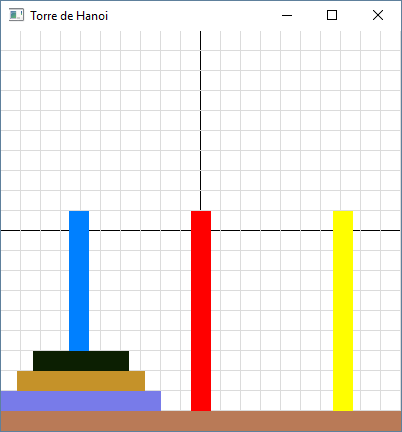
\includegraphics[scale=0.3]{img/hanoi_4a}
    \caption{Resolução da Torre de Hanói para 3 discos.} 
  \end{subfigure}
  ~
  \begin{subfigure}[t]{.25\textwidth}
    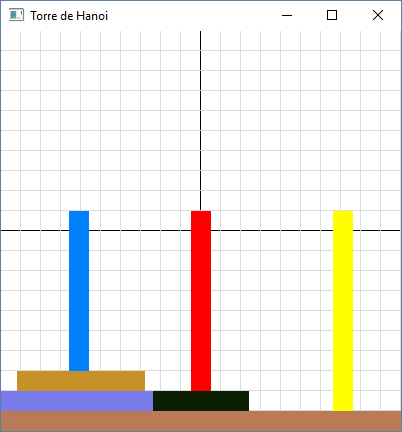
\includegraphics[scale=0.3]{img/hanoi_4b}
    \caption{Mova disco 1 de A para B.} 
  \end{subfigure}
  ~
  \begin{subfigure}[t]{.25\textwidth}
    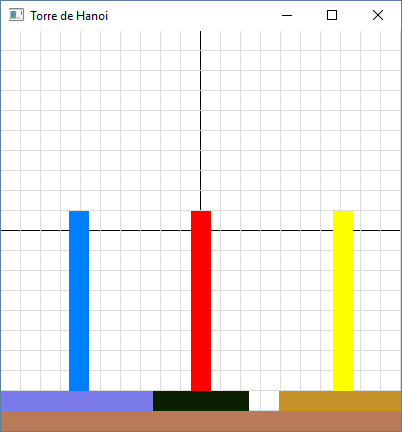
\includegraphics[scale=0.3]{img/hanoi_4c}
    \caption{Mova disco 2 de A para C.} 
  \end{subfigure}
  ~
  \begin{subfigure}[t]{.25\textwidth}
    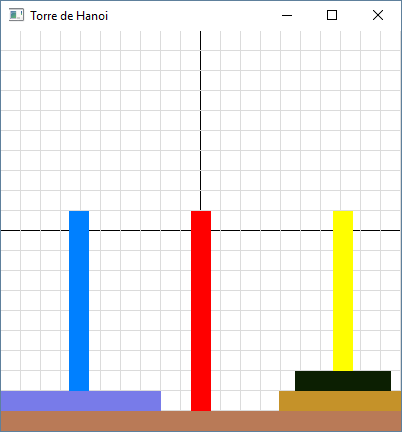
\includegraphics[scale=0.3]{img/hanoi_4d}
    \caption{Mova disco 1 de B para C.} 
  \end{subfigure}
  ~
  \begin{subfigure}[t]{.25\textwidth}
    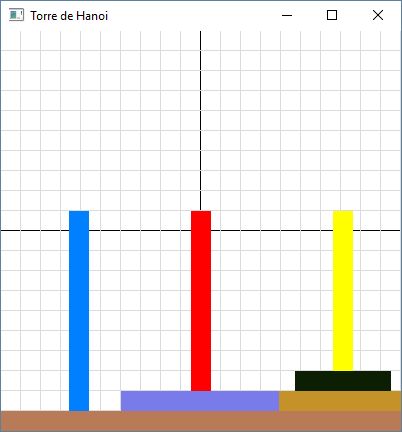
\includegraphics[scale=0.3]{img/hanoi_4e}
    \caption{Mova disco 3 de A para B.} 
  \end{subfigure}
  ~
  \begin{subfigure}[t]{.25\textwidth}
    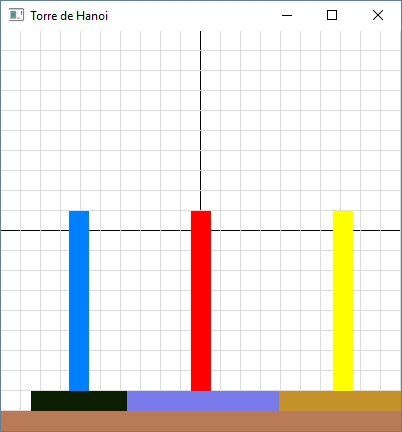
\includegraphics[scale=0.3]{img/hanoi_4f}
    \caption{Mova disco 1 de C para A.} 
  \end{subfigure}
  ~
  \begin{subfigure}[t]{.25\textwidth}
    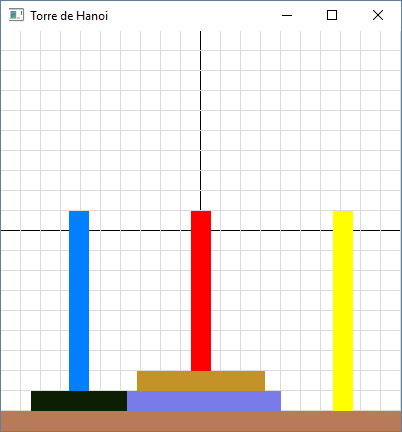
\includegraphics[scale=0.3]{img/hanoi_4g}
    \caption{Mova disco 2 de C para B.} 
  \end{subfigure}
  ~
  \begin{subfigure}[t]{.25\textwidth}
    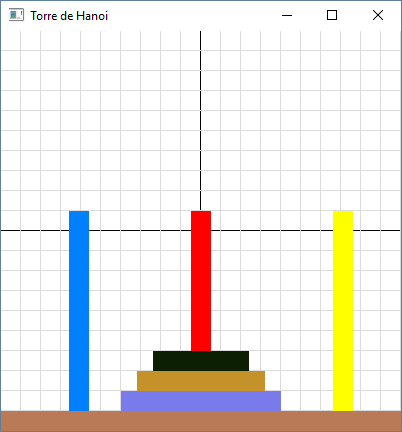
\includegraphics[scale=0.3]{img/hanoi_4h}
    \caption{Mova disco 1 de A para B.} 
  \end{subfigure}

  \caption{Solução da torre de Hanói para 3 discos: a) Início; b) Passo 1; c) Passo 2; d) Passo 3; e) Passo 4; f) Passo 5; g) Passo 6; h) Torre solucionada.} \label{fig:hanoicompleto}
\end{figure}
\lstinputlisting[style=code, label=lst:hanoi_3]{cpp/hanoi_4.cpp}















% \section{Práticas sugeridas pela \playAPC} \label{sec:enunciados}
% Baseado nos tópicos mais recorrentes da matéria inicial dos cursos de computação, explicado na Seção \ref{sec:projeto}, foram feitos 24 exercícios no total, separados por tópicos. Todos os exercícios, juntamente com sua solução, podem ser consultados no Apêndice \ref{appendix:apostila}. Neste Apêndice, ainda são encontrado mais 3 exercícios extras, que abordam todos os tópicos juntos.

% \subsection{Tipo de dados e estruturas de controle}

% \begin{renumerate}
% \item
% %   Exiba um plano cartesiano de -100 a 100 com espaçamento de 5 unidades.
% %   \label{ex:cap01_ex1}

% %   \begin{figure}[H]
% %     \centering
% %     \begin{subfigure}[t]{0.2\textwidth}
% %         \centerline{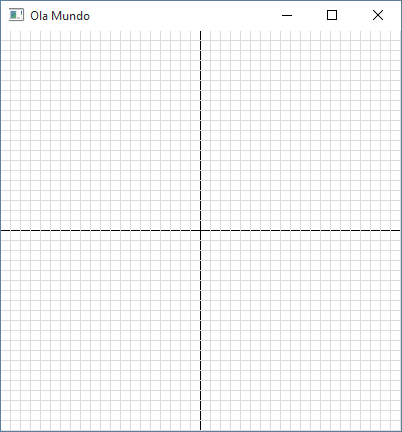
\includegraphics[width=.9\textwidth]{img/cap1_ex1.png}}
% %         \caption{Visualização de todo plano cartesiano.}
% %         \label{fig:cap01_ex1}
% %     \end{subfigure}
% %     ~
% %     \begin{subfigure}[t]{0.65\textwidth}
% %         \centerline{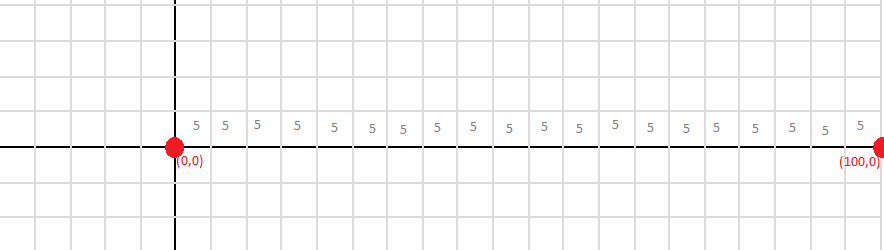
\includegraphics[width=.9\textwidth]{img/cap1_ex1_b.png}}
% %         \caption{De (0,0) até (100,0), existem 20 quadrados com 5 unidades de tamanho.}
% %         \label{fig:cap01_ex1}
% %     \end{subfigure}
% %     \caption{Plano cartesiano de -100 à 100: a) Todo plano; b) Parte do plano.}
% % \end{figure}


% \item \label{ex:cap01_ex2}
%   % Exiba um boneco palito.
  

%   % \begin{figure}[H]
%   %   \centerline{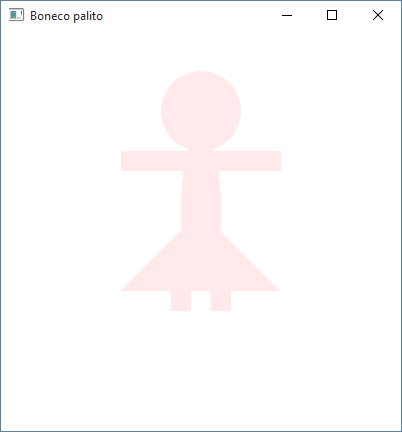
\includegraphics[width=.25\textwidth]{img/cap1_ex3.png}}
%   %   \caption{Boneco Palito.}
%   %   \label{fig:cap01_ex2}
%   % \end{figure}

% \item
%   % Exiba a estrela de Davi.
%   % \label{ex:cap01_ex3}

%   % \begin{figure}[H]
%   %   \centerline{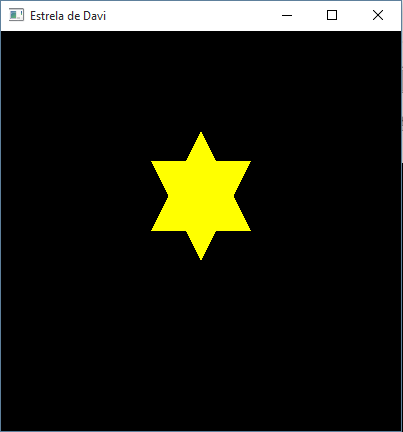
\includegraphics[width=.25\textwidth]{img/cap1_ex2.png}}
%   %   \caption{Estrela de Davi.}
%   %   \label{fig:cap01_ex3}
%   % \end{figure}

%   \item
%   % Escreva um programa que solicite do usuário um raio de um círculo e exiba um quadrado inscrito neste círculo.
%   % \label{ex:cap01_ex8}

%   % \begin{figure}[H]
%   %   \centerline{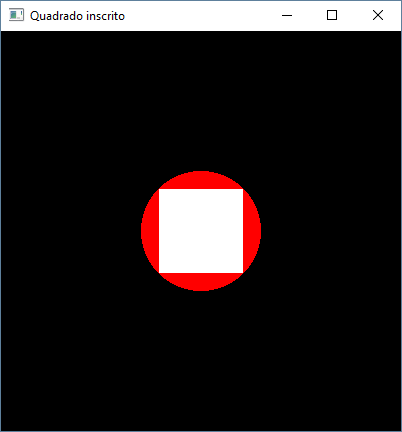
\includegraphics[width=.3\textwidth]{img/cap1_ex21}}
%   %   \caption{Quadrado inscrito em um círculo.}
%   %   \label{fig:cap01_ex8}
%   % \end{figure}


%   \item
%   %  Escreva um programa que solicita do usuário um raio, a posição do centro de uma circunferência e a posição de um ponto qualquer. Exiba a cena e indique no título da janela se o ponto está dentro ou fora da circunferência.

%   %  \begin{figure*}[!htb]
%   %   \centering
%   %   \begin{subfigure}[t]{0.3\textwidth}
%   %       \centerline{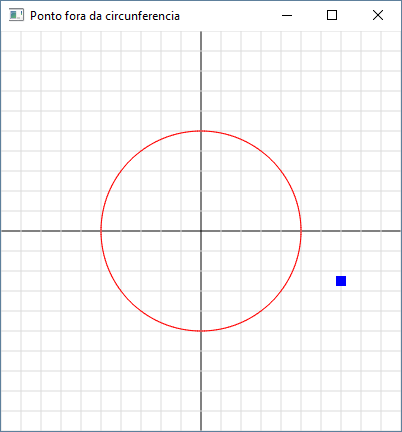
\includegraphics[width=.9\textwidth]{img/cap1_ex22}}
%   %       \caption{Ponto está fora da circunferência.}
%   %       \label{fig:cap01_ex22a}
%   %   \end{subfigure}
%   %   ~
%   %   \begin{subfigure}[t]{0.3\textwidth}
%   %       \centerline{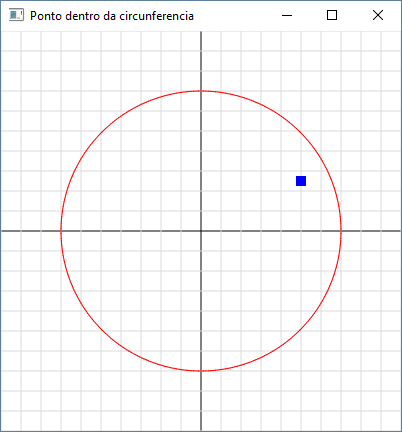
\includegraphics[width=.9\textwidth]{img/cap1_ex22b}}
%   %       \caption{Ponto está dentro da circunferência.}
%   %       \label{fig:cap01_ex22b}
%   %   \end{subfigure}
%   %   \caption{Verificação se ponto está dentro ou fora da circunferência: a) Fora; b) Dentro.}
%   % \end{figure*}

%   % \label{ex:cap01_ex22}

% \item
% %   Escreva um programa que receba do usuário um valor de ângulo em graus e um valor de raio. Converta para radianos o ângulo e exiba uma reta com o raio fornecido pelo usuário e pinte-a de acordo com as seguintes regras:
% %     \begin{itemize}
% %     \item
% %     Se a reta pertencer ao \emph{primeiro} quadrante, pinte-a de vermelho
% %     \item
% %     Se a reta pertencer ao \emph{segundo} quadrante, pinte-a de verde
% %     \item
% %     Se a reta pertencer ao \emph{terceiro} quadrante, pinte-a de azul
% %     \item
% %     Se a reta pertencer ao \emph{quarto} quadrante, pinte-a de preto
% %     \end{itemize}
% %     \label{ex:cap01_ex4}

% %   \begin{figure*}[h!]
% %     \centering
% %     \begin{subfigure}[t]{0.2\textwidth}
% %         \centerline{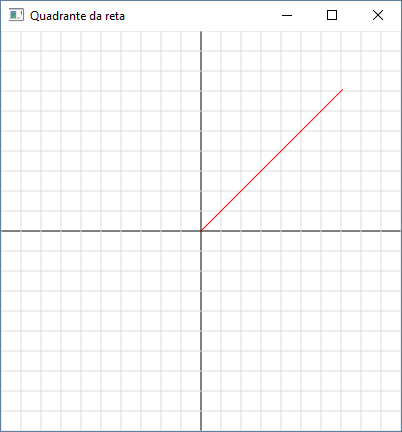
\includegraphics[width=.9\textwidth]{img/cap1_ex4}}
% %         \caption{Reta pertencente ao primeiro quadrante.}
% %         \label{fig:cap01_ex4a}
% %     \end{subfigure}
% %     ~
% %     \begin{subfigure}[t]{0.2\textwidth}
% %         \centerline{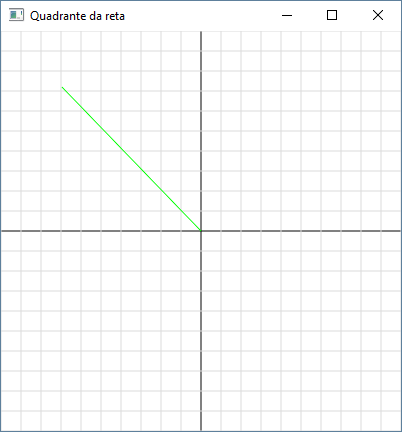
\includegraphics[width=.9\textwidth]{img/cap1_ex4b}}
% %         \caption{Reta pertencente ao segundo quadrante.}
% %         \label{fig:cap01_ex4b}
% %     \end{subfigure}
% %     ~
% %     \begin{subfigure}[t]{0.2\textwidth}
% %         \centerline{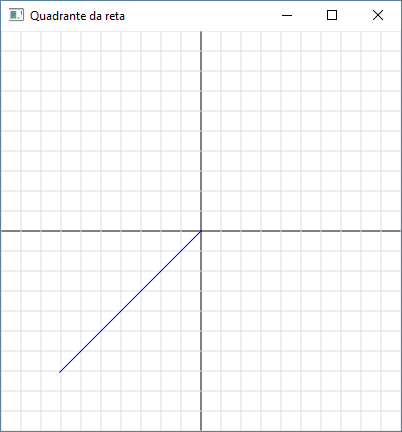
\includegraphics[width=.9\textwidth]{img/cap1_ex4c}}
% %         \caption{Reta pertencente ao terceiro quadrante.}
% %         \label{fig:cap01_ex4c}
% %     \end{subfigure}
% %     ~
% %     \begin{subfigure}[t]{0.2\textwidth}
% %         \centerline{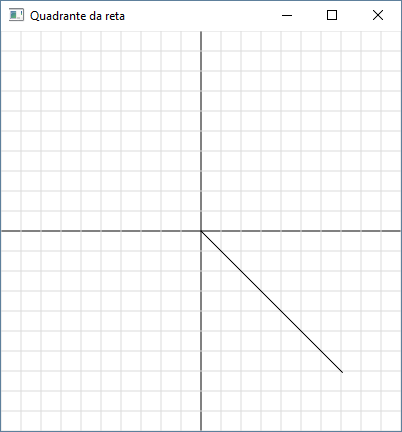
\includegraphics[width=.9\textwidth]{img/cap1_ex4d}}
% %         \caption{Reta pertencente ao quarto quadrante.}
% %         \label{fig:cap01_ex4d}
% %     \end{subfigure}
% %     \caption{Identificação de quadrante: a) Primeiro quadrante; b) Segundo quadrante; c) Terceiro quadrade; d) Quarto quadrante.}
% % \end{figure*}

% \item

% % Escreva um programa em C que solicita três pontos A, B e C ao usuário, e verifica se esses valores satisfazem a condição de existência do triângulo. Caso essa condição seja satisfeita, exiba esse triângulo e escreva no título da janela se o triângulo é equilátero, isósceles ou escaleno [dica: não usar a função CriaTriangulo()].

% %   \begin{figure}[H]
% %     \centering
% %     \begin{subfigure}[t]{0.3\textwidth}
% %         \centerline{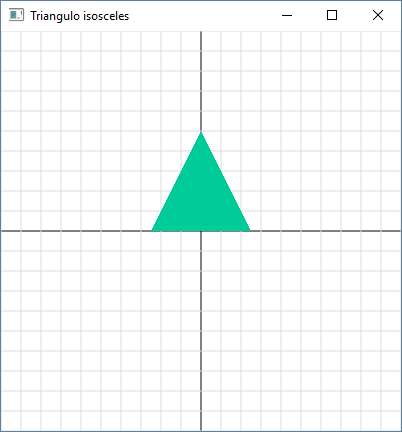
\includegraphics[width=.9\textwidth]{img/cap1_ex23}}
% %         \caption{Triângulo isósceles.}
% %         \label{fig:cap01_ex23a}
% %     \end{subfigure}
% %     ~
% %     \begin{subfigure}[t]{0.3\textwidth}
% %         \centerline{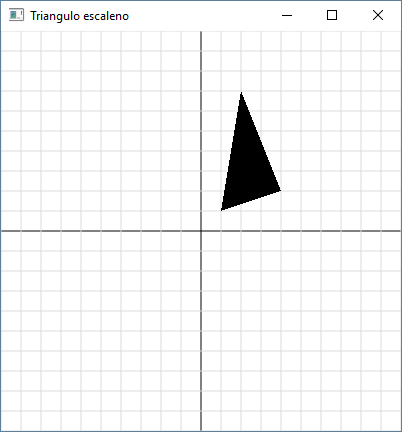
\includegraphics[width=.9\textwidth]{img/cap1_ex23b}}
% %         \caption{Triângulo escaleno.}
% %         \label{fig:cap01_ex23b}
% %     \end{subfigure}
% %     ~
% %     \begin{subfigure}[t]{0.3\textwidth}
% %         \centerline{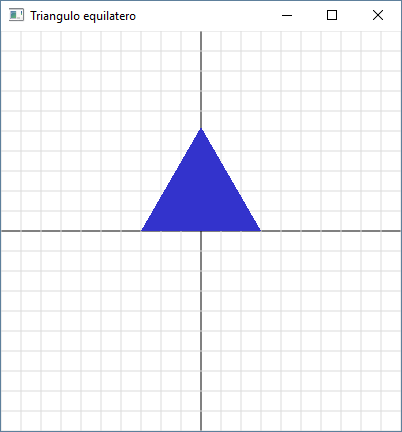
\includegraphics[width=.9\textwidth]{img/cap1_ex23c}}
% %         \caption{Triângulo equilátero.}
% %         \label{fig:cap01_ex23c}
% %     \end{subfigure}
% %     \caption{Existência de triângulos: a) Isósceles; b) Escaleno; c) Equilátero.}
% % \end{figure}

% % \label{ex:cap01_ex23}

% \item
%   % Exiba um carrinho se movendo de $-100$ à $100$.
%   % \label{ex:cap01_ex6}

%   % \begin{figure}[H]
%   %   \centerline{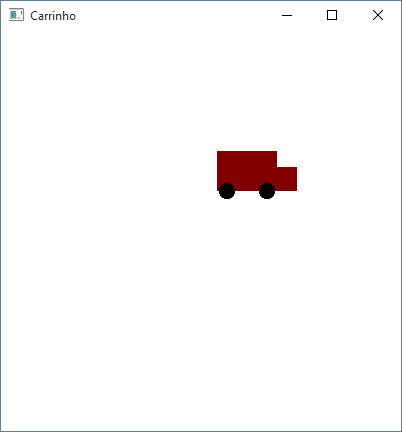
\includegraphics[width=.3\textwidth]{img/cap1_ex5.png}}
%   %   \caption{Carro se movendo da posição -100 até a posição 100.}
%   %   \label{fig:cap01_ex6}
%   % \end{figure}

% \item
%   % Construa um moinho de vento e coloque apenas as hélices para girar.
%   % \label{ex:cap01_ex7}

%   % \begin{figure}[H]
%   %   \centerline{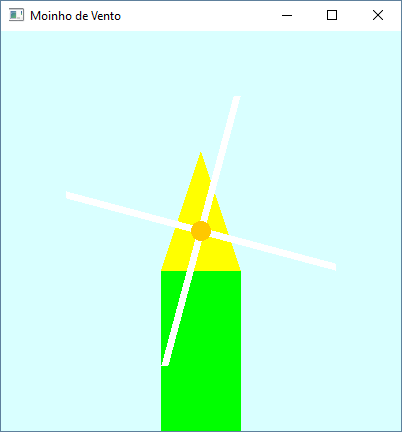
\includegraphics[width=.3\textwidth]{img/cap1_ex7.png}}
%   %   \caption{Moinho de vento.}
%   %   \label{fig:cap01_ex7}
%   % \end{figure}

% \item
%   % Escreva um programa utilizando a playAPC que simule simultaneamente o movimento da Terra ao redor do Sol e o movimento da Lua ao redor da Terra. Considere que as trajetórias de ambas são elípticas. No caso da Terra, o Sol é um dos focos e no caso da Lua, a Terra é um dos focos. Não é necessário simular a proporção real entre os semieixos maiores (a) da Lua e da Terra, nem a excentricidade (e) das duas trajetórias. Encontre empiricamente valores de (a) e (e) de forma que seja possível observar trajetórias elípticas. Simule, porém, a proporção real entre os movimento de translação da Terra e da Lua.
%   % \label{ex:cap01_ex24}

%   % \begin{figure}[H]
%   %   \centerline{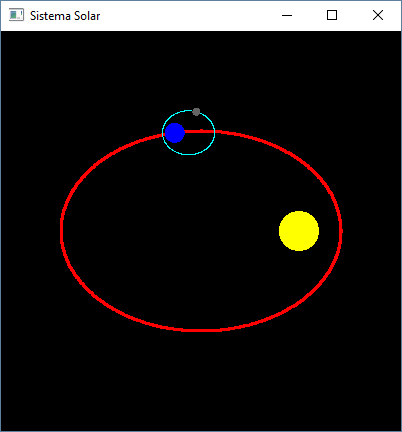
\includegraphics[width=.3\textwidth]{img/cap1_ex24.png}}
%   %   \caption{Sistema solar.}
%   %   \label{fig:cap01_ex24}
%   % \end{figure}

% \item
% %   Sabe-se que a equação da espiral hiperbólica pode ser defina por
% % \begin{equation} \label{eq:espiral}
% %   \begin{matrix}
% %   x & = & a \cos(\theta) \\ 
% %   y & = & a \sin(\theta)
% %   \end{matrix}.
% % \end{equation}
% %   onde $a$ é a assíntota para y e $\theta$ o ângulo equivalente ao ângulo em coordenadas polares. Para $a \gets 100$ e $\theta \in (0, 4\pi)$, desenhe duas espirais hiperbólicas calculando seus pontos como é descrito na Equação \ref{eq:espiral}. Para ponto $p$ em $(x,y)$ de uma das hiperbólica, o ponto $p$ da outra espiral deve estar posicionado em $(-x,-y)$.

% %   \label{ex:cap01_ex5}

% %   \begin{figure*}[!htp]
% %     \centering
% %     \begin{subfigure}[t]{0.3\textwidth}
% %         \centerline{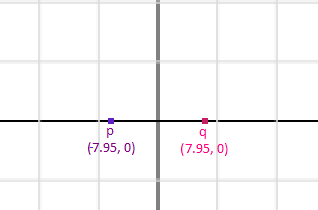
\includegraphics[width=.9\textwidth]{img/cap1_ex6}}
% %         \caption{Posição inicial aproximada de ambas as espirais.}
% %         \label{fig:cap01_ex6a}
% %     \end{subfigure}
% %     ~
% %     \begin{subfigure}[t]{0.3\textwidth}
% %         \centerline{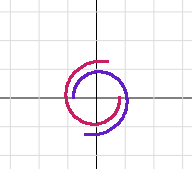
\includegraphics[width=.9\textwidth]{img/cap1_ex6b}}
% %         \caption{100º iteração no processo de criação das espirais.}
% %         \label{fig:cap01_ex6b}
% %     \end{subfigure}
% %     ~
% %     \begin{subfigure}[t]{0.3\textwidth}
% %         \centerline{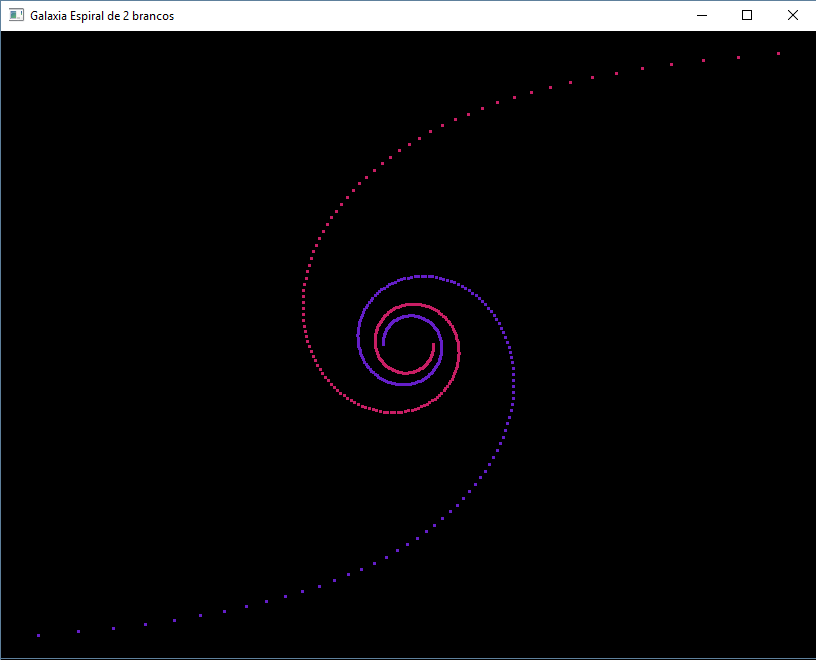
\includegraphics[width=.9\textwidth]{img/cap1_ex6c}}
% %         \caption{Espirais completas.}
% %         \label{fig:cap01_ex6c}
% %     \end{subfigure}
% %     \caption{Espiral hiperbólica: a) Primeira iteração; b) Centésima iteração; c) Espirais.}

% % \end{figure*}


%   \item
%   % Crie uma animação em que o Mário deve começar no canto esquerdo da tela e seu objetivo é andar até o canto direito da tela. Porém, haverão dois canos que serão posicionados aleatoriamente no meio do caminho, forçando o Mário a pulá-los para não colidir com eles. 
%   % Para criar a animação de andar, altere as imagens do retângulo onde será desenhado o Mario com a função \emph{AssociaImagem} e, após essa chamada, utilize a função \emph{Desenha1Frame} para renderizar a troca de imagens.

%   % Para simplificação do problema, considere que o Mário, ao realizar o pulo, ele deva executar meia trajetória circular, onde $\theta$ varia de $\pi$ até $0$ e o raio do pulo seja de $40$ unidades.
%   % \label{ex:cap01_ex25}

%   % \begin{figure}[H]
%   %   \centering
%   %   \begin{subfigure}[t]{0.3\textwidth}
%   %       \centerline{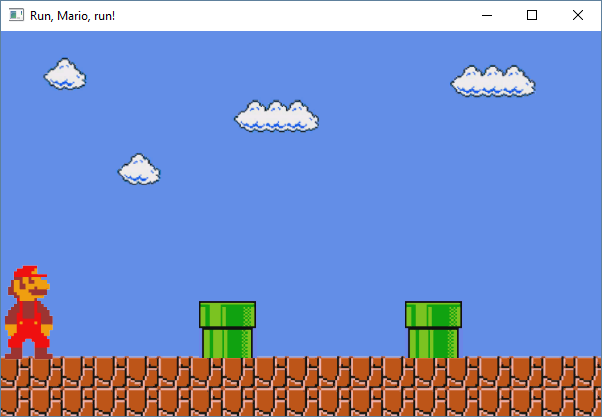
\includegraphics[width=.9\textwidth]{img/cap1_ex25}}
%   %       \caption{Começo da animação.}
%   %       \label{fig:cap01_ex6a}
%   %   \end{subfigure}
%   %   ~
%   %   \begin{subfigure}[t]{0.3\textwidth}
%   %       \centerline{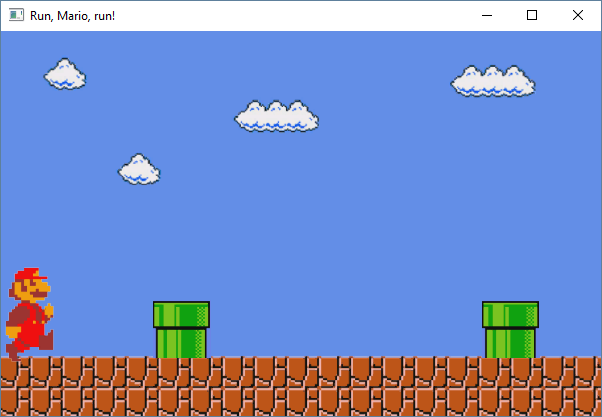
\includegraphics[width=.9\textwidth]{img/cap1_ex25b}}
%   %       \caption{Parte 1 da animação do Mário.}
%   %       \label{fig:cap01_ex6b}
%   %   \end{subfigure}
%   %   ~
%   %   \begin{subfigure}[t]{0.3\textwidth}
%   %       \centerline{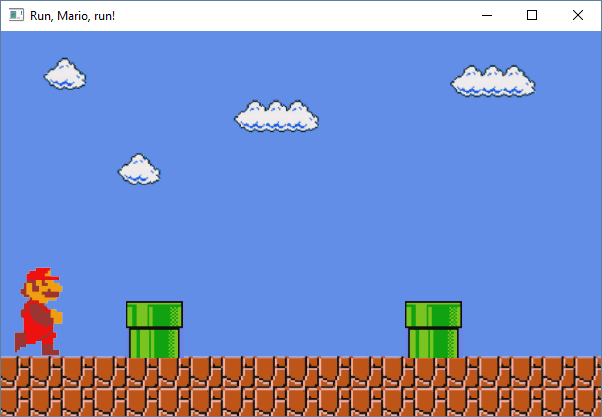
\includegraphics[width=.9\textwidth]{img/cap1_ex25c}}
%   %       \caption{Parte 2 da animação do Mário.}
%   %       \label{fig:cap01_ex6c}
%   %   \end{subfigure}
%   %   ~
%   %   \begin{subfigure}[t]{0.3\textwidth}
%   %       \centerline{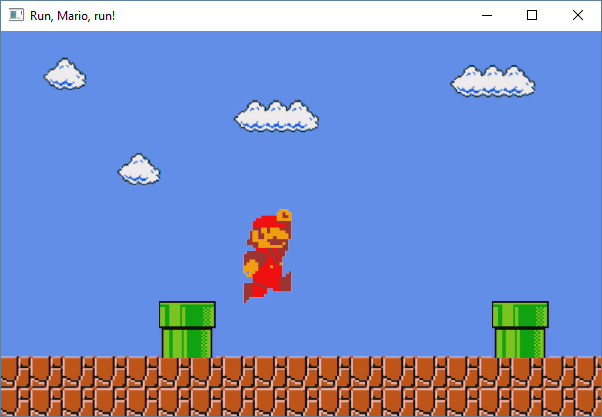
\includegraphics[width=.9\textwidth]{img/cap1_ex25d}}
%   %       \caption{Mário pulando.}
%   %       \label{fig:cap01_ex6c}
%   %   \end{subfigure}
%   %   \caption{Animação do Mário: a) Início; b) e c) Mário andando; d) Mário pulando.}
%   % \end{figure}

% \end{renumerate}

% \subsection{Vetores e Matrizes}

% \begin{renumerate}
% \item
%   % Exiba o gráfico do polinômio $-x^3$ para $-50 \leq x \leq 50$.
%   % \label{ex:cap02_ex1}

%   % \begin{figure}[ht]
%   %   \centerline{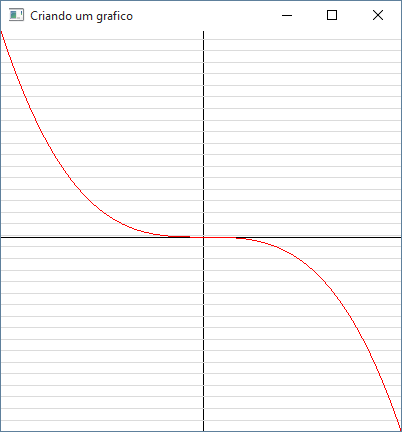
\includegraphics[width=.3\textwidth]{img/cap2_ex8.png}}
%   %   \caption{Gráfico do polinômio $-x^3$.}
%   %   \label{fig:cap02_ex1}
%   % \end{figure}

% \item
% %   Escreva uma programa que solicita ao usuário 20 componentes RGB do tipo int entre 0 e 255 que são armazenadas em três vetores R, G e B. Em seguida, os valores de cada vetor são filtrados por meio da filtragem de média móvel central, como indica a Equação \ref{eq:filtro} e o resultado é armazenado em três novos vetores Rf, Gf, Bf. O tamanho da janela de filtragem é fixo e igual a 3. 

% %   \label{ex:cap02_ex26}

% % \begin{equation} \label{eq:filtro}
% % \begin{matrix}
% % Rf[i] = & \frac{R[i-1] + R[i] + R[i+1]}{3}\\ 
% % Gf[i] = & \frac{G[i-1] + G[i] + G[i+1]}{3}\\ 
% % Bf[i] = & \frac{B[i-1] + B[i] + B[i+1]}{3}
% % \end{matrix}
% % \end{equation}
% % \equationset{Filtragem dos componentes \emph{RGB} do componente \emph{i} com janela de filtragem igual a 3}

% %   Exiba graficamente dois vetores coloridos, um composto pelas componentes RGB originais e outro pelas componentes RfGfBf filtradas. No final, o programa deve calcular também a distância euclidiana média entre os dois vetores RGB e RfGfBf, como indica a Equação \ref{eq:distancia}.

% %   \begin{equation} \label{eq:distancia}
% %   \frac{1}{n}\sum_{i = 0}^{n}\sqrt{(R[i] - Rf[i])^{2} + (G[i] - Gf[i])^{2} + (B[i] - Bf[i])^{2}}
% % \end{equation}
% % \equationset{Cálculo da distância euclidiana média}

% % \begin{figure}[H]
% %     \centerline{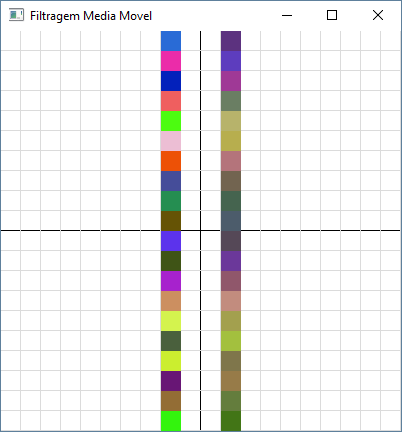
\includegraphics[width=.3\textwidth]{img/cap2_ex26.png}}
% %     \caption{À esquerda, 20 quadrados com componentes RGB fornecidos pelo usuário. À direita, aplicação do filtro de média móvel central em cada quadrado.}
% %     \label{fig:cap02_ex26}
% %   \end{figure}

% \item
%   % O jogo da vida é um autômato celular que simula a alteração e mudanças de grupos de seres vivos. Foi criado pelo matemático John Horton Conway na década de 70. Extremamente útil para diversas áreas da ciência, este autômato possui quatro regras simples:
%   % \begin{enumerate}
%   %   \item Qualquer célula viva com menos de dois vizinhos vivos morre de solidão
%   %   \item Qualquer célula viva com mais de três vizinhos vivos morre de superpopulação
%   %   \item Qualquer célula morta com exatamente três vizinhos vivos se torna uma célula viva
%   %   \item Qualquer célula viva com dois ou três vizinhos vivos continua no mesmo estado para a próxima geração
%   % \end{enumerate}
  
%   % Mostre graficamente o jogo da vida para uma matriz com 17 linhas e 17 colunas onde a população inicial estará \emph{VIVA} para as seguintes posições na matriz:
%   % $$
%   %   (1,5), (2,5), (3,5), (3,6), (5,1), (5,2), (5,3), (5,6), (5,7), (6,3), (6,5), (6,7), (7,5), (7,6)
%   % $$
%   % \label{ex:cap02_ex2}

%   %    \begin{figure}[H]
%   %   \centering
%   %   \begin{subfigure}[t]{0.27\textwidth}
%   %       \centerline{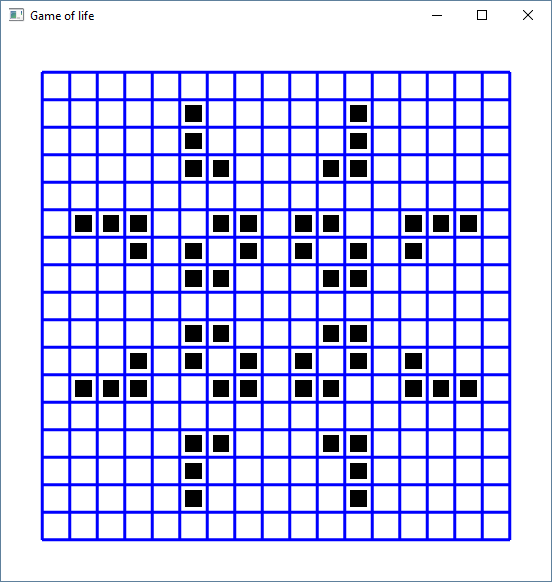
\includegraphics[width=.9\textwidth]{img/cap2_ex9.png}}
%   %       \caption{1ª geração.}
%   %       \label{fig:cap03_ex9a}
%   %   \end{subfigure}
%   %   ~
%   %   \begin{subfigure}[t]{0.27\textwidth}
%   %       \centerline{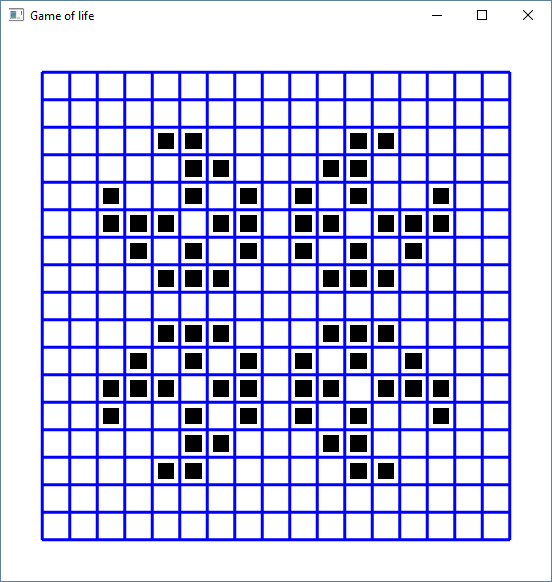
\includegraphics[width=.9\textwidth]{img/cap2_ex9b.png}}
%   %       \caption{2ª geração.}
%   %       \label{fig:cap03_ex9a}
%   %   \end{subfigure}
%   %   ~
%   %   \begin{subfigure}[t]{0.27\textwidth}
%   %       \centerline{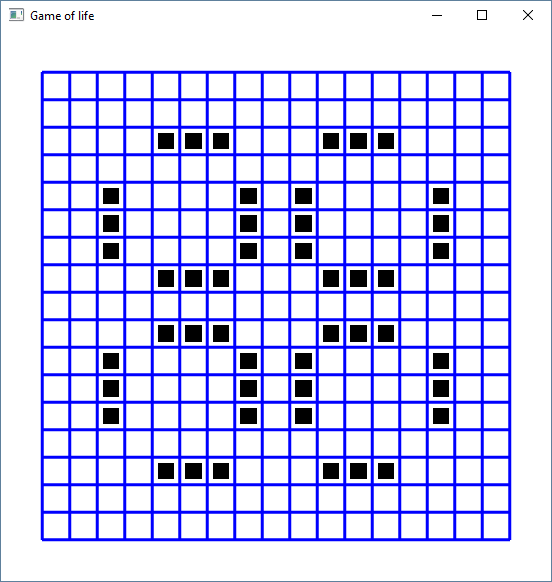
\includegraphics[width=.9\textwidth]{img/cap2_ex9c.png}}
%   %       \caption{3ª geração.}
%   %       \label{fig:cap03_ex9a}
%   %   \end{subfigure}
%   %   \caption{Jogo da vida: a) Primeira geração; b) Segunda geração; c) Terceira geração.}
%   % \end{figure}

%   \item
% % Implementar o filtro de média móvel para uma matriz M de inteiros (de 0 a 255) com 3 planos RGB, cada um com 100 linhas e 100 colunas.
% % A matriz a ser filtrada é a imagem uma imagem BMP do Mario. Ela deve ser lida e em seguida mostrada na tela do computador. A imagem filtrada deve igualmente ser apresentada na tela do computador.
% %   \label{ex:cap02_ex27}

% %   \begin{figure}[H]
% %     \centerline{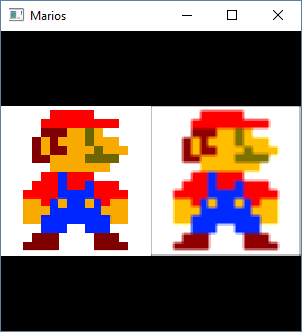
\includegraphics[width=.3\textwidth]{img/cap2_ex27.png}}
% %     \caption{Filtro Motion Blur.}
% %     \label{fig:cap02_ex27}
% %   \end{figure}

% \item
% % O jogo batalha naval é um jogo de tabuleiro no qual os jogadores devem adivinhar em quais posições do tabuleiro estão localizados os navios do adversário. Ganha aquele que derrubar todos os navios.
% % Implemente o jogo batalha naval utilizando a \playAPC{}, utilizando as seguintes premissas:
% % \begin{itemize}
% %   \item O tabuleiro será 9x9;
% %   \item Posicione arbitrariamente 10 navios sobre este tabuleiro, sendo 3 navios com tamanho igual a 3, 3 navios com tamanho igual a 2 e 4 navios com tamanho igual a 1;
% %   \item Não pode posicionar um navio onde já existir outro navio e não pode posicionar o navio imediatamente do lado de outro navio: deve existir pelo menos um espaço vazio entre os dois navios;
% %   \item Os navios podem estar nas verticais e nas horizontais, não nas diagonais;
% %   \item Se um navio de tamanho igual a 1 for atingido, fica indicado no lugar que o navio foi derrubado;
% %   \item Se um navio de tamanho igual a 2 ou 3 for atingido, deve ficar indicado que o navio foi atingido, porém não foi derrubado. Somente quando todas as peças deste navio forem atingidas é que deve-se indicar o navio foi derrubado;
% %   \item Se o usuário escolheu uma posição do tabuleiro onde não há navio, deve ficar indicado que o usuário não atingiu água e;
% %   \item O jogo deve avisar ao usuário quando ele conseguir derrubar todos os 10 navios.
% % \end{itemize}

% %     \begin{figure}[H]
% %     \centering
% %     \begin{subfigure}[t]{0.3\textwidth}
% %         \centerline{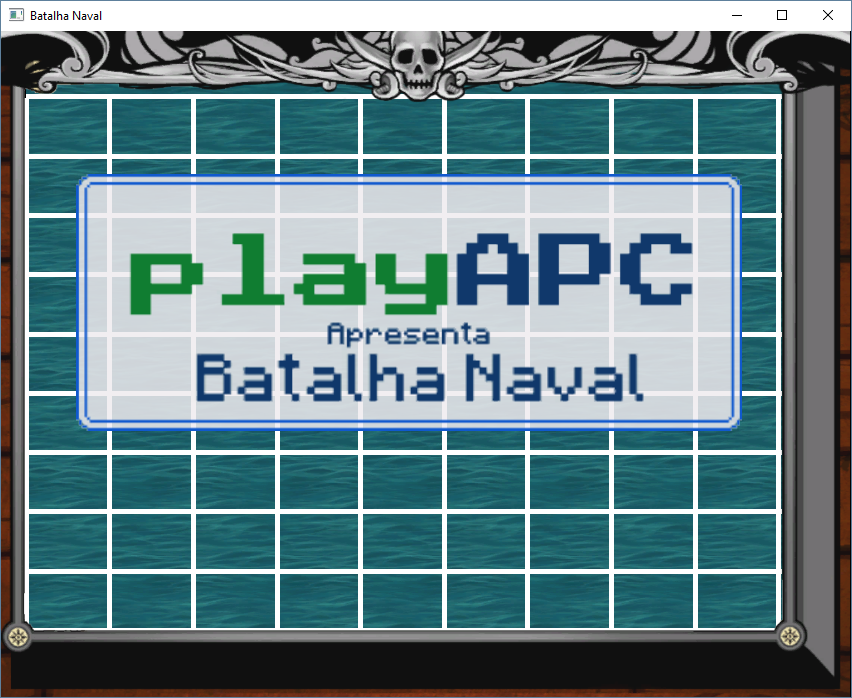
\includegraphics[width=.9\textwidth]{img/cap2_ex29.png}}
% %         \caption{Tela inicial.}
% %         \label{fig:cap03_ex26}
% %     \end{subfigure}
% %     ~
% %     \begin{subfigure}[t]{0.3\textwidth}
% %         \centerline{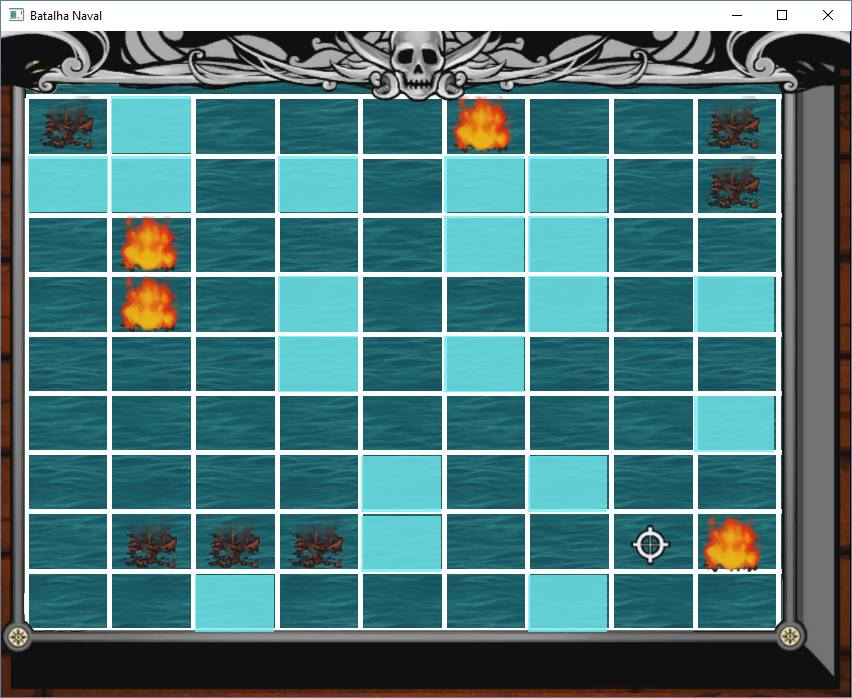
\includegraphics[width=.9\textwidth]{img/cap2_ex29b.png}}
% %         \caption{Decorrer do jogo: há navios atingidos e navios derrubados.}
% %         \label{fig:cap03_ex26b}
% %     \end{subfigure}
% %     ~
% %     \begin{subfigure}[t]{0.3\textwidth}
% %         \centerline{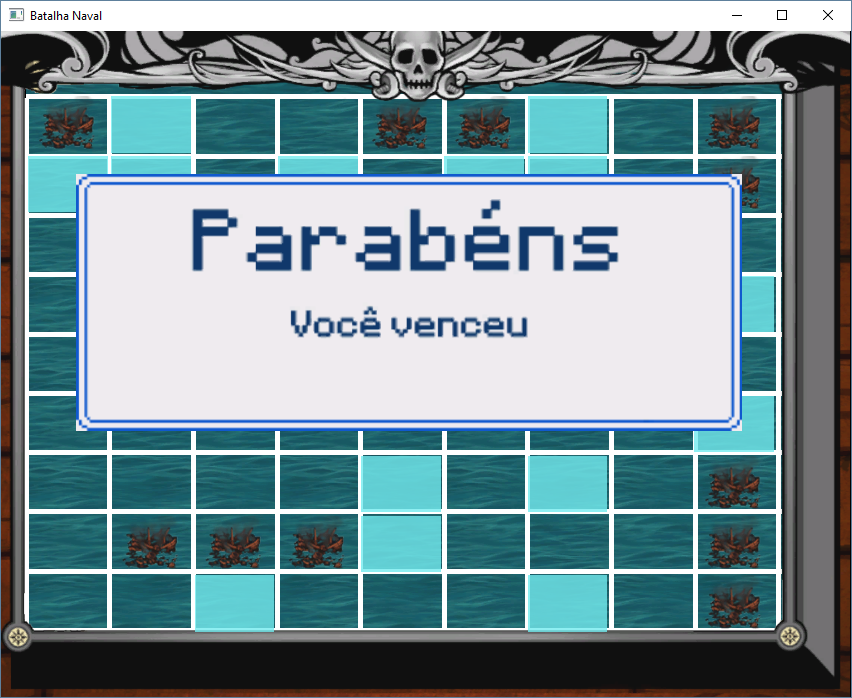
\includegraphics[width=.9\textwidth]{img/cap2_ex29c.png}}
% %         \caption{Fim do jogo.}
% %         \label{fig:cap03_ex26c}
% %     \end{subfigure}
% %     \caption{Batalha Naval: a) Início; b) Decorrer do jogo; c) Fim do jogo.}
% %   \end{figure}

% \end{renumerate}

% \subsection{Subalgoritmos}

% \begin{renumerate}
% \item
%   % Crie dois retângulos e posicione-os aleatoriamente em $x$. Coloque uma circunferência no topo do primeiro retângulo e receba do usuário dois valores: ângulo e velocidade. Dado estes valores, calcule e exiba a trajetória balística da circunferência sendo lançada para o outro retângulo. Exiba mensagem caso o usuário consiga acertar o prédio ou não e, em seguida, caso o usuário deseje jogar novamente, sorteie novas posições para os retângulos e execute novamente o procedimento de pedir valores do usuário e exibir a trajetória balística.

%   % \begin{figure}[ht]
%   %   \centerline{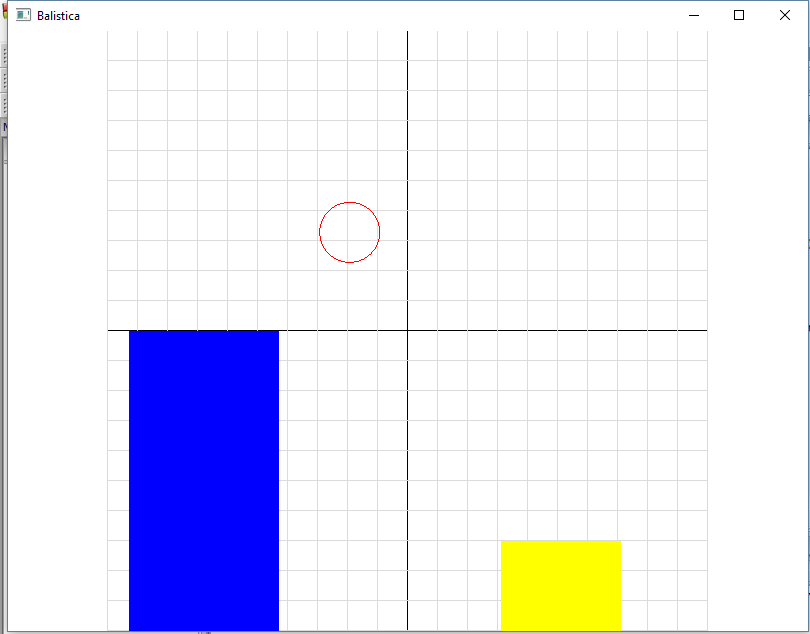
\includegraphics[width=.25\textwidth]{img/cap3_ex12.png}}
%   %   \caption{Lançador Balístico.}
%   %   \label{fig:cap03_ex2}
%   % \end{figure}

%   % \label{ex:cap03_ex1}

%   \item
%   % Baseado no exercício anterior, faça o Wolverine ser lançado de um prédio, dado um ângulo e uma velocidade inicial, com o objetivo de atacar o Magneto. Se não atingir o Magneto, os dois inimigos se encaram. Se atingir o Magneto, faça o Magneto contra-atacar o Wolverine, lançando o mutante em uma trajetória retilínia na direção contrária ao ataque.


%   %  \begin{figure}[H]
%   %   \centering
%   %   \begin{subfigure}[t]{0.25\textwidth}
%   %       \centerline{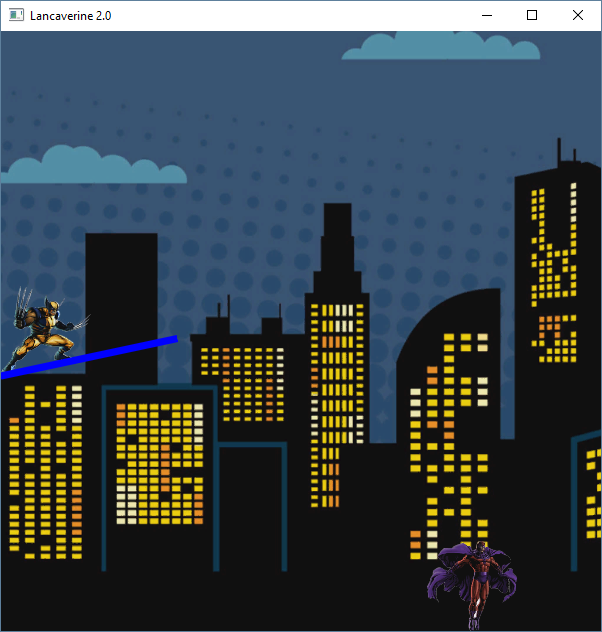
\includegraphics[width=.9\textwidth]{img/cap3_ex27}}
%   %       \caption{Determinação do ângulo.}
%   %       \label{fig:cap03_ex27a}
%   %   \end{subfigure}
%   %   \hfill
%   %   \begin{subfigure}[t]{0.25\textwidth}
%   %       \centerline{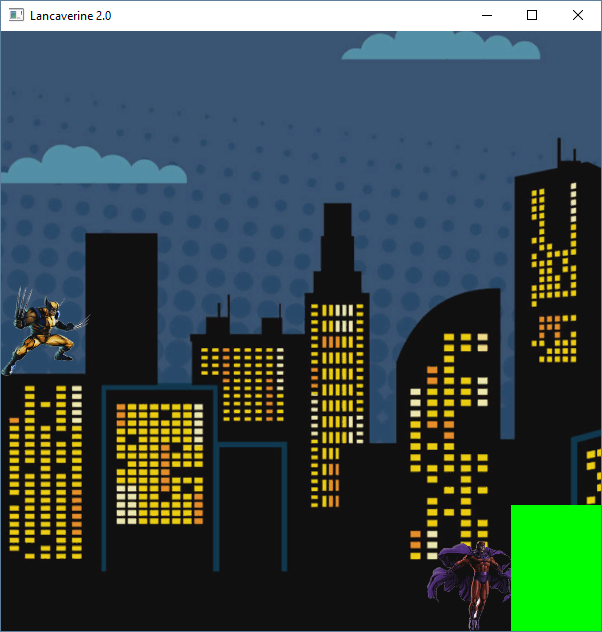
\includegraphics[width=.9\textwidth]{img/cap3_ex27b}}
%   %       \caption{Determinação da velocidade inicial.}
%   %       \label{fig:cap03_ex27b}
%   %   \end{subfigure}
%   %   \hfill
%   %   \begin{subfigure}[t]{0.25\textwidth}
%   %       \centerline{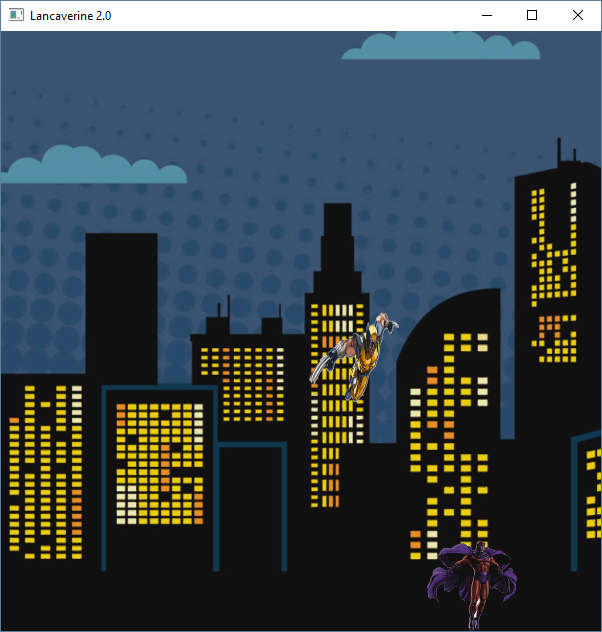
\includegraphics[width=.9\textwidth]{img/cap3_ex27c}}
%   %       \caption{Wolverine sendo lançado.}
%   %       \label{fig:cap03_ex27c}
%   %   \end{subfigure}
%   %   \hfill
%   %   \begin{subfigure}[t]{0.25\textwidth}
%   %       \centerline{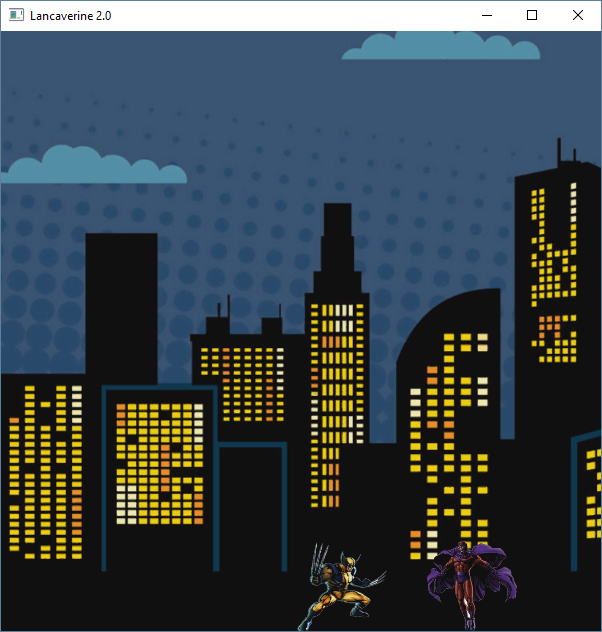
\includegraphics[width=.9\textwidth]{img/cap3_ex27d}}
%   %       \caption{Wolverine e Magneto se encarando.}
%   %       \label{fig:cap03_ex27d}
%   %   \end{subfigure}
%   %   ~
%   %   \begin{subfigure}[t]{0.25\textwidth}
%   %       \centerline{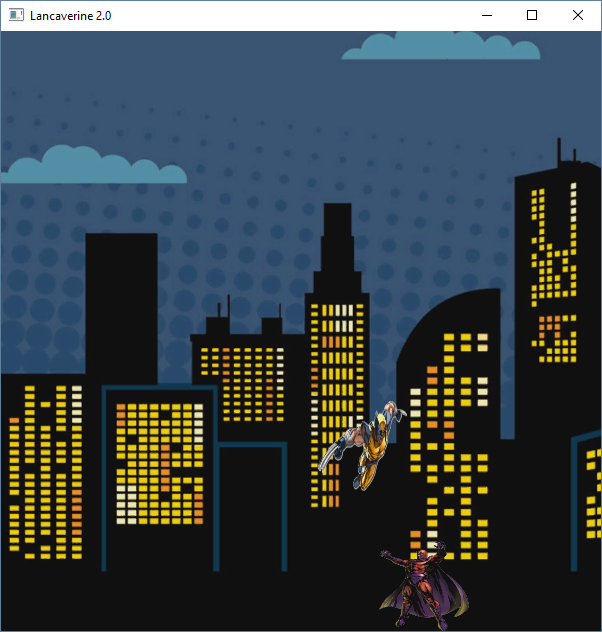
\includegraphics[width=.9\textwidth]{img/cap3_ex27e}}
%   %       \caption{Wolverine sendo lançado pelo Magneto.}
%   %       \label{fig:cap03_ex27e}
%   %   \end{subfigure}

%   %   \caption{Lançaverine: a) Ângulo de lançamento; b) Velocidade inicial; c) Wolverine percorrendo trajetória; d) Caso quando Wolverine não acerta o Magneto; e) Caso quando Wolverine acerta o Magneto.}

%   % \end{figure}

%   % \label{ex:cap03_ex27} 
  
% \item
%   % Snake foi um jogo que começou no console Atari, em 1976, e foi popularizado nos anos 90 quando a Nokia começou a colocar o jogo em seus celulares. 
  
%   % O jogador controla uma cobra, que é representada por um quadrado no começo, e, a cada novo alimento que a cobra ingere, ela aumenta em um quadrado o seu tamanho, aumentando gradativamente a dificuldade do jogo. Se a cobra atingir a parede, ela morre. Se a cobra atingir o próprio corpo, ela também morre.

%   % Dado estas regras, crie uma versão do jogo Snake utilizando a \playAPC.

%   % \label{ex:cap03_ex2}

%   % \begin{figure}[H]
%   %   \centerline{\includegraphics[width=.25\textwidth]{img/cap3_ex10.png}}
%   %   \caption{Jogo Snake.}
%   %   \label{fig:cap03_ex2}
%   % \end{figure}

% \end{renumerate}

% \subsection{Recursão} \label{ex:recursao}

% \begin{renumerate}

% \item
%   % Construa uma árvore binária recursiva onde o usuário oferece altura, profundidade e ângulo entre ramos. A árvore deverá ser construída tanto para o lado esquerdo, com ângulo entre os galhos de $\theta$ fornecida pelo usuário, quanto para o lado direito, com ângulo $-\theta$.
%   % \label{ex:cap04_ex2}

%   % \begin{figure}[H]
%   %   \centerline{\includegraphics[width=.3\textwidth]{img/cap4_ex17.png}}
%   %   \caption{Árvore Binária com altura $30$, ângulo $25$º e profundidade $6$.}
%   %   \label{fig:cap04_ex2}
%   % \end{figure}

% \item
%   % Torre de Hanói é um jogo matemático onde seu objetivo é passar os discos de uma torre $A$ para uma torre $B$, utilizando uma torre $C$ como auxiliar. Ele segue as seguintes regras:
%   % \begin{enumerate}
%   %   \item Só pode mover um disco de cada vez
%   %   \item Só pode mover o disco que estiver mais acima de uma torre e deve-se colocar no topo de outra torre
%   %   \item Não é permitido colocar um disco de tamanho maior em cima de um disco de tamanho menor
%   % \end{enumerate}

%   % Ilustre a resolução da torre de Hanói para uma quantidade de 5 discos ou menos.
%   % \label{ex:cap04_ex1}

%   % \begin{figure}[H]
%   %   \centerline{\includegraphics[width=.3\textwidth]{img/cap4_ex13.png}}
%   %   \caption{Solucionador da torre de Hanói.}
%   %   \label{fig:cap04_ex1}
%   % \end{figure}

% \item
%   % Sabe-se que a curva de Koch começa sendo construída com um segmento de reta de tamanho $\frac{n}{3}$. Na extremidade deste primeiro segmento, desenha-se outro segmento de reta de tamanho $\frac{n}{3}$, porém com uma curvatura de $60º$ em relação ao primeiro. Na extremidade deste segundo segmento, desenha-se outra curva de reta de tamanho $\frac{n}{3}$, mas agora com a curvatura de $120º$ em relação ao primeiro. Por fim, desenha-se outro segmento de reta de tamanho $\frac{n}{3}$ na extremidade do terceiro segmento, sem diferença de curvatura.

%   %   \begin{enumerate}[label=(\alph*)]
%   %     \item Exiba a curva de Koch de ordem $i$ com tamanho $n$ igual à $180$ unidades centrada na posição $(-100, 0)$. 
        
%   %       (NOTA: a partir de um certo nível de recursão, é possível que a divisão dos segmentos de retas comecem a dividir pixels, tornando inviável a visualização)

%   %     Como sugestão, a Listagem \ref{func:koch} exemplifica um cabeçalho da função \emph{koch}, onde seu primeiro argumento é o ponto de origem, seu segundo argumento é o tamanho do segmento de reta, seu terceiro argumento é a inclinação do segmento e seu quarto argumento é a ordem da curva. A função retorna o segundo ponto da reta naquele nível de recursão que deverá ser criada.

%   %     \begin{lstlisting}[caption=Header da função koch, label={func:koch},numbersep=0pt,resetmargins=true, language=C++]
%   %     Ponto koch (Ponto from, double len, double theta, int order)
%   %     \end{lstlisting}

%   %       \label{ex:cap04_ex3a}

%   %         \begin{figure}[H]
%   %         \centering
%   %         \begin{subfigure}[t]{0.3\textwidth}
%   %             \centerline{\includegraphics[width=.9\textwidth]{img/cap4_ex14}}
%   %             \caption{Curva de Koch de ordem $1$.}
%   %             \label{fig:cap03_ex14a}
%   %         \end{subfigure}
%   %         \hfill
%   %         \begin{subfigure}[t]{0.3\textwidth}
%   %             \centerline{\includegraphics[width=.9\textwidth]{img/cap4_ex14b}}
%   %             \caption{Curva de Koch de ordem $2$.}
%   %             \label{fig:cap03_ex14b}
%   %         \end{subfigure}
%   %         \hfill
%   %         \begin{subfigure}[t]{0.3\textwidth}
%   %             \centerline{\includegraphics[width=.9\textwidth]{img/cap4_ex14c}}
%   %             \caption{Curva de Koch de ordem $3$.}
%   %             \label{fig:cap03_ex14c}
%   %         \end{subfigure}
%   %         \hfill
%   %         \begin{subfigure}[t]{0.3\textwidth}
%   %             \centerline{\includegraphics[width=.9\textwidth]{img/cap4_ex14d}}
%   %             \caption{Curva de Koch de ordem $6$.}
%   %             \label{fig:cap03_ex14d}
%   %         \end{subfigure}
          
%   %         \caption{
%   %           \label{fig:koch}%
%   %           Curva de Koch: a) Ordem 1; b) Ordem 2; c) Ordem 3; d) Ordem 6.
%   %         }

%   %       \end{figure}

%   % \label{ex:cap03_ex27}

%   %     \item Utilize a curva de Koch criada no item anterior para criar outras duas curvas, com uma diferença de angulação: a primeira curva será criada da mesma maneira no item anterior; a segunda curva será inclinada em $120º$ e; a terceira curva será inclinada em $-120º$. 

%   %     As Figuras \ref{fig:flocos} ilustram as três retas, onde a primeira curva, com inclinação $0º$, está representada em vermelho, a segunda, com inclinação de $120º$ está representada em verde e a terceira curva, com inclinação $-120º$ está representada em azul.
%   %     \label{ex:cap04_ex3b}

%   %     \begin{figure}[H]
%   %         \centering
%   %         \begin{subfigure}[t]{0.3\textwidth}
%   %             \centerline{\includegraphics[width=.9\textwidth]{img/cap4_ex15}}
%   %             \caption{Floco de neve de ordem $1$.}
%   %             \label{fig:cap04_ex15a}
%   %         \end{subfigure}
%   %         \hfill
%   %         \begin{subfigure}[t]{0.3\textwidth}
%   %             \centerline{\includegraphics[width=.9\textwidth]{img/cap4_ex15b}}
%   %             \caption{Floco de neve de ordem $2$.}
%   %             \label{fig:cap04_ex15b}
%   %         \end{subfigure}
%   %         \hfill
%   %         \begin{subfigure}[t]{0.3\textwidth}
%   %             \centerline{\includegraphics[width=.9\textwidth]{img/cap4_ex15c}}
%   %             \caption{Floco de neve de ordem $3$.}
%   %             \label{fig:cap04_ex15c}
%   %         \end{subfigure}
%   %         \hfill
%   %         \begin{subfigure}[t]{0.3\textwidth}
%   %             \centerline{\includegraphics[width=.9\textwidth]{img/cap4_ex15d}}
%   %             \caption{Floco de neve de ordem $6$.}
%   %             \label{fig:cap04_ex15d}
%   %         \end{subfigure}

%   %         \caption{
%   %           \label{fig:flocos}%
%   %           Floco de neve: a) Ordem 1; b) Ordem 2; c) Ordem 3; d) Ordem 6.
%   %         }

%   %       \end{figure}
%   %   \end{enumerate}

%   % \label{ex:cap04_ex3}

% \item
%  %  A curva de Sierpiński é uma curva do tipo \emph{space-filling curve}, a qual significa que ela tenta ocupar todo espaço disponível sem ser cruzar. Ela pode ser implementada utilizando quatro funções mutuamente recursivas, \emph{A, B, C} e \emph{D}. A Figura \ref{fig:cap04_ex16} ilustra essa curva com as 4 curvas básicas. A curva A está representado em vermelho, a curva B em verde, a curva C em azul e a curva D em amarelo, sendo as curvas que conectam estas 4 curvas básicas representadas em preto.

%  %   \begin{figure}[H]
%  %    \centerline{\includegraphics[width=1.0\textwidth]{img/cap4_ex16.png}}
%  %    \caption{Curva de Sierpiński de ordem $1$ com ângulo de $45º$.}
%  %    \label{fig:cap04_ex16}
%  %  \end{figure}


%  % O programa inicia com uma curva básica \emph{S} dada pelo padrão A 
%  %      \begin{tikzpicture}
%  %        \draw[thick,->] (0.0,0.30) -- (0.30,0.0);
%  %      \end{tikzpicture}
%  %      , B
%  %      \begin{tikzpicture}
%  %        \draw[thick,->] (0.30,0.30) -- (0.0,0.0);
%  %      \end{tikzpicture}
%  %      , C
%  %      \begin{tikzpicture}
%  %        \draw[thick,->] (0.30,0.0) -- (0.0,0.30);
%  %      \end{tikzpicture}
%  %      e D
%  %      \begin{tikzpicture}
%  %        \draw[thick,->] (0.0,0.0) -- (0.30,0.30);
%  %      \end{tikzpicture}
%  %      . As setam indicam a virada do ângulo que as retas \emph{fecham} os desenhos das funções.
%  %  \begin{itemize}
%  %    \item
%  %      A curva A é dada pelo padrão A
%  %      \begin{tikzpicture}
%  %        \draw[thick,->] (0.0,0.30) -- (0.30,0.0);
%  %      \end{tikzpicture}
%  %      , B
%  %      \begin{tikzpicture}
%  %        \draw[thick,->] (0.0,0.0) -- (0.30,0.0);
%  %      \end{tikzpicture}
%  %      , D
%  %      \begin{tikzpicture}
%  %        \draw[thick,->] (0.0,0.0) -- (0.30,0.30);
%  %      \end{tikzpicture}
%  %      A
%  %    \item
%  %      A curva B é dada pelo padrão B
%  %      \begin{tikzpicture}
%  %        \draw[thick,->] (0.30,0.30) -- (0.0,0.0);
%  %      \end{tikzpicture}
%  %      , C
%  %      \begin{tikzpicture}
%  %        \draw[thick,->] (0.30,0.30) -- (0.30,0.0);
%  %      \end{tikzpicture}
%  %      , A
%  %      \begin{tikzpicture}
%  %        \draw[thick,->] (0.0,0.30) -- (0.30,0.0);
%  %      \end{tikzpicture}
%  %      B
%  %    \item
%  %      A curva C é dada pelo padrão C
%  %      \begin{tikzpicture}
%  %        \draw[thick,->] (0.30,0.0) -- (0.0,0.30);
%  %      \end{tikzpicture}
%  %      , D
%  %      \begin{tikzpicture}
%  %        \draw[thick,->] (0.30,0.0) -- (0.0,0.0);
%  %      \end{tikzpicture}
%  %      , B
%  %      \begin{tikzpicture}
%  %        \draw[thick,->] (0.30,0.30) -- (0.0,0.0);
%  %      \end{tikzpicture}
%  %      C
%  %    \item
%  %      A curva D é dada pelo padrão D
%  %      \begin{tikzpicture}
%  %        \draw[thick,->] (0.0,0.0) -- (0.30,0.30);
%  %      \end{tikzpicture}
%  %      , A
%  %      \begin{tikzpicture}
%  %        \draw[thick,->] (0.30,0.0) -- (0.30,0.30);
%  %      \end{tikzpicture}
%  %      , C
%  %      \begin{tikzpicture}
%  %        \draw[thick,->] (0.30,0.0) -- (0.0,0.30);
%  %      \end{tikzpicture}
%  %      D
%  %  \end{itemize}
%  %  Considere o ângulo de inclinação da curva de Sierpiński como $45º$, ou seja, as retas desenhadas tem uma inclinação de $45º$ entre si. Considere também que a curva tenha uma altura $h$ de $40$ unidades e que, caso a ordem de recusão $n$ seja maior que $0$, a altura será determinada por $\frac{h}{n^{2}}$. A criação das curvas se inicia no ponto $p$ em $(-70, 100)$. 

%  %  Considere que a Listagem \ref{func:sier} seja a função que calcula o próximo ponto baseando no ângulo de inclinação e desenha esta reta. Estes fatores são passados de acordo com a Listagem \ref{func:mainsier}.
%  %  \label{ex:cap04_ex4}

%  %  \begin{lstlisting}[caption={Função para conectar próxima curva}, style=tuto, , label={func:sier}] 
%  %      Ponto reta(int fator, int h, Ponto p) {
%  %        // ang é para multiplicar por 45 graus
%  %        Ponto p1;
%  %        double ar = fator * 45.0 * PI/180;

%  %        p1.x = p.x + h*cos(ar);
%  %        p1.y = p.y + h*sin(ar);
%  %        CriaReta(p,p1);
%  %        Grafite(2);
%  %        Pintar(0,0,255);
%  %        return p1;
%  %      }
%  %      \end{lstlisting}

%  %    \begin{lstlisting}[caption={Função main Curva de Sierpiński}, style=tuto, label={func:mainsier}] 
%  %      int main() {

%  %        Ponto p;
%  %        int   k; 
%  %        float   h = 40;

%  %        printf("Insira a ordem para a criacao das curvas: ");
%  %        scanf("%d", &k);

%  %        p.x = -70; p.y = 100; //ordem=1 cabe todo na tela


%  %        MostraPlanoCartesiano(10);
%  %        AbreJanela(800,600, "Curvas de Sierpinski");
%  %        PintarFundo(255, 255, 255);


%  %        if (k>0) h /= k*k;
%  %        p = A(k,h, p); 
%  %        p = reta(7,h, p); //calcula o proximo ponto onde a outra reta deve comecar

%  %        p = B(k,h, p); 
%  %        p = reta(5,h, p); 

%  %        p = C(k,h, p); 
%  %        p = reta(3,h, p);

%  %        p = D(k,h, p); 
%  %        p = reta(1,h, p);

%  %        Desenha();

%  %        return 0;
%  %      }
%  %      \end{lstlisting}

%  %  Implemente as funções $A$, $B$, $C$ e $D$ da curva de Sierpiński.

%  %  \begin{figure*}[!htp]
%  %          \centering
%  %          \begin{subfigure}[t]{0.45\textwidth}
%  %              \centerline{\includegraphics[width=.9\textwidth]{img/cap4_ex16b}}
%  %              \caption{Curva de Sierpiński de ordem $2$.}
%  %              \label{fig:cap03_ex14a}
%  %          \end{subfigure}
%  %          \hfill
%  %          \begin{subfigure}[t]{0.45\textwidth}
%  %              \centerline{\includegraphics[width=.9\textwidth]{img/cap4_ex16c}}
%  %              \caption{Curva de Sierpiński de ordem $3$.}
%  %              \label{fig:cap03_ex14b}
%  %          \end{subfigure}
          
%  %          \caption{
%  %            \label{fig:koch}%
%  %            Curva de Sierpiński: a) Ordem 2; b) Ordem 3.
%  %          }

%  %        \end{figure*}
  
% \end{renumerate}



% Além do  próprio aluno conseguir desenhar  formas geométricas convexas
% com  \texttt{CriaPoligono}, a  \playCB{}  disponibiliza outras  formas
% geométricas:      \emph{triângulo     isósceles},     \emph{quadrado},
% \emph{retângulo},  \emph{círculo}, \emph{circunferência},  \emph{elipse}, \emph{ponto}
% e  \emph{reta}.  A  partir  destas formas  básicas,  é possível  criar
% outras formas geométricas mais complexas incluindo as não convexas.

% Na \playCB{} existe o conceito de \emph{grupo}. Grupo é um conjunto de
% ``geometrias;'' se  aplicarmos uma determinada  transformação linear a
% um grupo, essa transformação é aplicada a todos os elementos do grupo.
% Um exemplo deste uso  está na Listagem~\ref{carro}. Esse exemplo exibe
% um carro, feito com três figuras geométricas, passando por trás de uma
% casa, feita com duas figuras geométricas. Cada um está dividido em sua
% própria  função, mas  isso  não  é sempre  necessário,  como mostra  a
% Listagem~\ref{solar},  onde cada planeta  é um  grupo distinto  que se
% move de forma independente.


% \section{Programação Orientada a Objetos}

% A orientação a objetos foi escolhida neste projeto devido a facilidade
% de abstrair os problemas da \acrfull{CG}. Desta forma, loop
% de renderização, limpeza de buffer ou detalhes de funcionamento da \acrshort{API}
% OpenGL~\cite{angel6th,cookbook,sb6,opengl8th,aot4,wikiogl}       foram
% encapsulados e foi criada uma interface com estes elementos de \acrshort{CG}, mas
% sem  o usuário  necessariamente  saber como  eles  funcionam.  Em  seu
% projeto, a arquitetura em camadas  foi escolhida devido por motivos de
% organização, que  tem como objetivo facilitar a  agilizar a manutenção
% do código~\cite{poo,poojs,poowong,poonirosh}.

% \subsection{Arquitetura em Camadas}
% De modo a descentralizar uma grande aplicação, é viável a busca de criação de métodos e classes que possam ter propósitos mais genéricos. Desta forma, cada componente presente em uma camada são auto-suficientes e sua comunicação entre outras camadas reduz-se a simples chamadas de métodos. Com isso, aumenta a reusabilidade e a manutenabilidade de um projeto~\cite{poo}. No caso da \playCB{}, caso fosse necessário mudar a API GLFW 2.7 para a GLFW 3.0, ou a GLUT, bastaria modificar a classe \emph{OpenglBase}, mantendo os métodos ou adicionando novos, se fosse o caso.

% A Fig.~\ref{fig:arq} ilustra esta arquitetura é utilizada e como cada camada se comunica.

% \begin{figure}[ht!]
% \centering  %\includegraphics[scale=0.5]{Arquitetura_PlayCB}
% \begin{tikzpicture}[>=stealth,scale=1.55]
% \draw (0,.5) rectangle (1,.8); \node at (.5,.65) 
%         {\tiny\texttt{\textbf{Interface}}};
% \draw (0,0) rectangle (1.5,.5);
% \node at (.75,.25) {\tiny\texttt{PlayCB}};

% \draw (2.7,.5) rectangle (4,.8); \node at (3.3,.65) 
%         {\tiny\texttt{\textbf{Negócios}}};
% \draw (2.7,0) rectangle (5.75,.5);
% \node at (4.125,.25) {\tiny\texttt{Evento Geometria Grupo}};

% \draw (6.75,.5) rectangle (7.75,.8); \node at (7.25,.65) 
%         {\tiny\texttt{\textbf{Dados}}};
% \draw (6.75,0) rectangle (8.25,.5);
% \node at (7.5,.25) {\tiny\texttt{OpenGL base}};

% \draw[->,blue] (1,.65) -- (2.7,.65);
% \draw[->,blue] (4,.65) -- (6.75,.65);
% \end{tikzpicture}
% \caption{Organização da arquitetura da \playCB}
% \label{fig:arq}
% \end{figure}

% \begin{itemize}
% \item A camada de interface é a comunicação entre o usuário e a API gráfica,
% que trata desde  a criação de objetos a serem exibidos  na tela até ao
% loop de renderização, todos estruturados de forma sequencial, em que o
% usuário  possa  escrever  um  programa  sem a  necessidade  de  ter  o
% conhecimento de orientação a objeto. Esta camada abrange o seguinte código fonte e o arquivo de cabeçalho, ambos de mesmo nome:
% 	\begin{enumerate}
% 		\item playcb
% 	\end{enumerate}

% \item A camada de  dados é responsável pela manipulação  da biblioteca GLFW,
% responsável  pela  criação de  janelas  com  o  contexto da  OpenGL  e
% gerencia  os eventos  para  renderização, sendo  chamada somente  pela
% camada de negócios. Esta camada abrange o seguinte código fonte e o arquivo de cabeçalho, ambos de mesmo nome:
% 	\begin{enumerate}
% 		\item OpenglBase
% 	\end{enumerate}

% \item A  camada  de  negócios  é  a camada  que  constrói  objetos,  realiza
% transformações  algébricas  e   gerencia  chamadas  para  controle  de
% renderização.  Grande parte do código fonte da \playCB{} se concentra nessa camada, pois esta abrange os seguintes códigos fontes e seus respectivos arquivos de cabeçalhos:
% 	\begin{enumerate}
% 		\item Grupo
% 		\item Evento
% 		\item PlanoCartesiano
% 		\item Geometria
% 			\begin{enumerate}
% 				\item Circulo
% 				\item Circunferencia
% 				\item Elipse
% 				\item Poligono
% 				\item Pontinho
% 				\item Reta
% 				\item Retangulo
% 				\item Triangulo
% 			\end{enumerate}
% 	\end{enumerate}
% \end{itemize}

% \subsection{Encapsulamento}
% Encapsulamento é um termo usado normalmente como sinônimo de ``esconder informação,'' mas não necessariamente de modo físico, e sim com interface com módulos bem definidos o qual o conhecimento de sua implementação não é necessária para a construção e abstração do programa que o usuário está construindo~\cite{poo}.

% Toda a camada de interface da \playCB{} se utiliza desta metodologia de projeto para simplificar o processo de criação de figuras geométricas e sua renderização, tendo o melhor exemplo nesta camada a função \emph{Desenha}, que esconde a informação de que esta função é responsável pelo loop de renderização.

% Não apenas na camda de interface, mas a comunicação entre camadas também, como é possível notar no diagrama da Figura ~\ref{fig:sequencia}.

% \begin{figure}[h!]
% 	\begin{center}
% 		\includegraphics[width=1.0\textwidth]{img/Sequencia_playcb}
% 	\end{center}
% 	\caption{Diagrama de Sequência da função \emph{AbreJanela}}
% 	\label{fig:sequencia}
% \end{figure}

% Para o funcionamento desta chamada de função \emph{AbreJanela}, a interface da playcb cria um objeto do tipo Evento, sendo esta classe responsável por gerenciar todos os eventos de input e renderização. Note que não há a necessidade de saber como é implementado este objeto para a main, tornando o próprio objeto \emph{Evento} independente de código, uma vez que sua funcionalidade foi abstraída para somente devolver ao usuário uma janela de contexto.

% \subsection{Herança}
% Uma vez que classes podem partilhar das mesmas características ou métodos, sendo estes métodos não necessariamente completamente idênticos em funcionalidades, herança é uma recurso em Orientação a Objetos com ênfase em reusabilidade~\cite{poo}.

% A \playCB{} utiliza este método com a classe Geometria, que possui métodos e atributos em comum com as subclasses Círculo, Circunferência, Polígono, Reta, Retângulo e Triângulo.
% \small
% \begin{lstlisting}%
% [caption={Descrição da classe Geometria}, label=geometria,
% emph={AbreJanela,PintarFundo,Ponto,CriaCircunferencia,CriaCirculo,CriaGrupo,%
% Pintar,Grafite,Move,Desenha,Desenha1Frame},
% emphstyle={\color{green!50!black}\bfseries},
% numbersep=.5mm]
% class Geometria{
%     protected:
%         GLfloat red, green, blue;
%         GLfloat grafite;
%         Geometria *prox;
%         GLuint textura;
%     public:
%         ///Métodos virtuais
%         virtual void RenderizaPontos() = 0; //Método para desenhar as geometrias, com glBegin() e glEnd()
%         ///Métodos em comum de todas as geometrias
%         void Cor(GLfloat red = 0, GLfloat green = 0, GLfloat blue = 0); //Define cores
%         void Grafite(GLfloat grafite = 1.0); //Define grossura da borda
%         void Agrupa(Geometria *prox); //Cria lista de geometrias
%         Geometria *getProx(); //Pega o próximo elemento da lista
%         GLuint getTextura(); //Retorna área alocada para textura
%         void setTextura(GLuint data); //Seta área alocada para textura
% };
% \end{lstlisting}
% \normalsize

% \subsubsection{Classes}
% Classe é uma definição de um tipo abstrato de dado, especificando sua implementação de forma total ou parcial. Um objeto é uma instância de uma classe, criado e manipulado somente em tempo de execução do programa~\cite{poo}. Subclasse são classes que herdam atributos ou métodos de outra classe, sendo esta abstrata ou não.

% As classes referente as geometrias que podem ser criadas com a \playCB{} se diferenciam no método \emph{RenderizaPontos()}, visto que esta classe é um método virtual. Cada uma utiliza a função da OpenGL \emph{glBegin()} e \emph{glEnd()}, a qual é especificada na sessão de Computação Gráfica.
% \begin{itemize}
% 	\item A classe \emph{Pontinho} é criada a partir de um único \emph{Ponto p} passado pelo usuário e utiliza como argumento para \emph{glBegin()} o \emph{GL\_POINTS}.
% 	\item A classe \emph{Reta} é criada a partir de dois pontos \emph{Ponto p1} e \emph{Ponto p2} passado pelo usuário e utiliza como argumento para \emph{glBegin()} o \emph{GL\_LINES}.
% 	\item A classe \emph{Poligono} é criada a partir de n pontos, agrupados em um deque, passado pelo usuário e utiliza como argumento para \emph{glBegin()} o \emph{GL\_POLYGON}.
% 	\item A classe \emph{Triangulo} é criada a partir de um único ponto \emph{Ponto p} de referência, que é o ponto do canto esquerdo inferior, um valor para a base e um valor para a altura passados pelo usuário e utiliza como argumento para \emph{glBegin()} o \emph{GL\_TRIANGLES}.
% 	\item A classe \emph{Retangulo}, que é a mesma utilizada para criar quadrados com \emph{CriaQuadrado}, é criada a partir de um único ponto \emph{Ponto p} de referência, que é o ponto do canto esquerdo inferior, um valor para a base e um valor para a altura passados pelo usuário e utiliza como argumento para \emph{glBegin()} o \emph{GL\_QUADS}.
% 	\item A classe \emph{Circulo} é criada a partir de um único ponto \emph{Ponto p} de referência, que é o ponto do centro do círculo e um valor o raio passados pelo usuário e utiliza como argumento para \emph{glBegin()} o \emph{GL\_TRIANGLE\_FAN}. Cada ponto do círculo é calculado a partir da fórmula:
		
% 		Para x é inicializado com o valor do raio e y inicializado com 0
% 		\begin{align*}
% 	        x = & x - y  \tan (\theta)  \cos(\theta) \\
% 	        y = & y + x  \tan (\theta)  \cos(\theta)
% 		\end{align*}

% 	\item A classe \emph{Circunferencia} é criada a partir de um único ponto \emph{Ponto p} de referência, que é o ponto do centro da circunferência e um valor o raio passados pelo usuário e utiliza como argumento para \emph{glBegin()} o \emph{GL\_LINE\_LOOP}. Cada ponto da circunferência é calculada da mesma forma que o círculo.
% \end{itemize}


% \section{Álgebra Linear}
% Álgebra linear é uma área da matemática derivada da geometria analítica no plano e espaço e busca a resolução de sistemas lineares, onde vetores podem ser reduzinos a polinômios, funções e outros elementos abstratos~\cite{labma}. Tal abstração é de suma importância para a computação gráfica, pois suas primitivas são representadas na forma de vetores e escalares.

% \subsection{Espaço Vetorial}
% Um espaço vetorial é definido por:
% \begin{itemize}
% 	\item um conjunto não vazio $V$, cujo os elementos são chamados de vetores
% 	\item conjunto numérico $K$, cujo elementos são chamados de escalares
% 	\item uma soma vetorial: operação que associa a cada dois vetores $ v, u in V $ um vetor $ v + u \in V $
% 	\item uma multiplicação por escalar: operação que associa a cada vetor $v \in V$ e um escalar $k \in K$ um vetor $kv \in V$
% \end{itemize}
% Baseado nesta definição~\cite{labma}, podemos aplicar este conceito nas transformações lineares que a \playCB{} utiliza em seu projeto.
% \subsection{Transformações lineares}
% Seja $V$ e $W$ dois espaços vetorais, define-se uma função de transformação linear $T$ como:
% 	\begin{equation*}
%     	T:V \rightarrow W
% 	\end{equation*}
% Onde, para cada elemento $v \in V$ e $w \in W$, teremos:
% 	\begin{equation*}
%     	w = T(v)
% 	\end{equation*}
% Baseado nesta definição~\cite{alT}, uma vez que os objetos da \playCB{} estão localizados em um plano 2D, foram implementadas as seguintes transformações: translação, rotação e escala.
% \subsubsection{Translação}
% Translação é um deslocamento de um ponto à outro ponto em um plano~\cite{transrot}. Dado o vetor de deslocamento $d$, calcula-se para todos os pontos da figura sua translação baseado na equação~\cite{angel6th}:
% 	\begin{equation*}
%     	T(v) = v + d
% 	\end{equation*}

% 	\begin{figure}[h!]
% 		\begin{center}
% 			\includegraphics[scale=0.75]{img/linear1}
% 		\end{center}
% 		\caption{Translação. (a) figura na posição original (b) figura transladada }
% 		\label{fig:linear1}
% 	\end{figure}

% A Figura~\ref{fig:linear1} ilustra este conceito em uma figura com três dimensões, tendo sua ideia também replicada em duas dimensões.

% \subsubsection{Rotação}
% Dado um ângulo $\Theta$, rotaciona-se a figura em torno da origem do sistema~\cite{transrot}. Uma vez que a \playCB{} utiliza um plano cartesiano 2D como sistema, de -100 à 100, sua origem encontra-se no centro $(0,0)$. Um ponto particular $(x,y)$ será rotacionado para a posição $(x',y')$ dado um ângulo $\Theta$. Este cálculo é feito da seguinte forma~\cite{angel6th}: 
% 	\begin{equation*}
%     	\begin{bmatrix}
% 			x'\\ 
% 			y'
% 		\end{bmatrix} 
% 		= 
% 		\begin{bmatrix}
% 			cos\Theta  & -sin\Theta \\ 
% 			sin\Theta& cos\Theta
% 		\end{bmatrix}
% 		\begin{bmatrix}
% 			x\\ 
% 			y
% 		\end{bmatrix}
% 	\end{equation*}

% 	\begin{figure}[h!]
% 		\begin{center}
% 			\includegraphics[scale=0.8]{img/linear2}
% 		\end{center}
% 		\caption{Rotação de um ponto e rotação de uma figura em um plano 2D }
% 		\label{fig:linear2}
% 	\end{figure}

% A Figura~\ref{fig:linear2} ilustra a rotação em torno do eixo y de um ponto e uma figura. A ilustração representa o que está implementado na \playCB{}.

% \subsubsection{Escala}
% Escala é uma transformação aplicada em um corpo não uniforme, que o faz maior ou menor. Dado duas constantes $\alpha$, uma vez que a \playCB{} trabalha somente no plano 2D, o cálculo de sua transformação de escala, para cada ponto, é feito da seguinte forma~\cite{aulaRalha}:
% \begin{equation*}
% 	\begin{bmatrix}
% 			x'\\ 
% 			y' \\
% 			1 \\
% 			1
% 		\end{bmatrix} 
% 		= 
%     \begin{bmatrix}
% 		 \alpha_x& 0 & 0 & 0 \\ 
% 		 0 & \alpha_y & 0 & 0\\ 
% 		 0& 0 & 1 & 0\\ 
% 		 0& 0 & 0 & 1
% 	\end{bmatrix}
% 	\begin{bmatrix}
% 			x\\ 
% 			y\\
% 			1\\
% 			1\\
% 		\end{bmatrix}
% \end{equation*}
	
% \begin{figure}[h!]
% 	\begin{center}
% 		\includegraphics[scale=0.8]{img/linear3}
% 	\end{center}
% 	\caption{Tranformação de escala em uma figura }
% 	\label{fig:linear3}
% \end{figure}

% A Figura~\ref{fig:linear3} ilustra um rediomensionamento de uma figura 3D, tendo sua ideia também replicada no plano 2D.

% \section{Computação Gráfica}
% \subsection{OpenGL}
% OpenGL é uma API para renderizar gráficos 3D utilizando procedimentos específicos do \emph{hardware} dedicado para este processo, a placa de vídeo (\emph{GPU}). A Figura ~\ref{fig:arqopengl} ilustra a arquitetura da OpenGL, exibindo a comunicação da \emph{CPU} e \emph{GPU}~\cite{johnnyartigo}. 
% \begin{figure}[h!]
% 	\begin{center}
% 		\includegraphics[scale=0.8]{img/opengl2}
% 	\end{center}
% 	\caption{Representação gráfica da arquitetura de uma aplicação utilizando a API OpenGL }
% 	\label{fig:arqopengl}
% \end{figure}

% A OpenGL assume que a alocação de memória responsável pela exibição de pixels na tela seja feita pelo sistema operacional, garantindo sua portabilidade para inúmeros sistemas, sendo somente responsável pela atualização do \emph{buffer} de memória gráfico, mais especificamente, o \emph{Frame Buffer}. A Figura ~\ref{fig:estadosbuffer} ilustra a máquina de estados responsável para a atualização deste \emph{buffer}~\cite{johnnyartigo}.
% \begin{figure}[h!]
% 	\begin{center}
% 		\includegraphics[scale=0.5]{img/opengl1}
% 	\end{center}
% 	\caption{Máquina de estados para atualização do \emph{Frame Buffer} }
% 	\label{fig:estadosbuffer}
% \end{figure}
% \subsection{GLU}
% GLU \emph{OpenGL Utility Library} é uma biblioteca que cria uma interface com a OpenGL. Ela possui um conjunto de funções de alto nível, como por exemplo transformações lineares, mapeamento da tela e algumas primitivas geométricas, sendo estas funções compatíveis com a versão 1.3 da OpenGL~\cite{glu}.
% \subsection{GLFW}
% GLFW 2.7 é uma API específica para o uso com a OpenGL feita com a linguagem C. Sua proposta é, além facilitar o gerenciamento de uma janela de contexto, incluir em suas funcionalidades:
% \begin{itemize}
% 	\item entrada de teclado, mouse e joystick
% 	\item maior precisão de tempo
% 	\item suporte a \emph{mult-threading}
% 	\item suporte de \emph{query} e uso de extensões da OpenGL
% 	\item suporte básico de carregamento de imagens
% \end{itemize}
% Baseado na proposta desta API~\cite{glfw}, a \playCB{} utiliza em sua camada de dados funções específicas da GLFW para o tratamento da janela de contexto, para o suporte a imagens e para o tratamento de entrada de teclado.
% \subsection{SOIL}
% EXPLICAR COMO A SOIL FOI UTILIZADA